\documentclass[8pt,xcolor*pst]{beamer}
%----------------------------------------------------------------------
%                     Chargement de quelques packages
%----------------------------------------------------------------------
% utile pou redaction, � enlever pour version d�finitive}
%\usepackage{showkeys}
% Pour les figures PS :
%\usepackage[pdftex]{graphicx}
%\usepackage[dvips]{graphicx}
\usepackage{graphicx}
% Pour traiter le PS :
\usepackage{psfrag}
% Pour faire des sous figures
\usepackage{subfigure}
\usepackage{rotating}
%pour certains tableaux
\usepackage{hhline}
%packages de math
\usepackage{amsmath}
\usepackage{amsthm}
\usepackage{amsfonts}
\usepackage{amssymb}
\usepackage{amsbsy}
\usepackage{stmaryrd} 
%\usepackage{subeqnarray}
%\usepackage{subeqnarray}
% pour la cesure des mots
%\usepackage[T1]{fontenc}
%\usepackage{inputenc}
\usepackage{textcomp}
%pour quelques symboles comme degr�
%\usepackage{inputenc}
%pour l'environnement remarque
%\usepackage{theorem}
%\usepackage{ntheorem}
%pour faire pleins de colonnes
\usepackage{multicol}
%pour faire des colonnes de tableau beau
\usepackage{tabularx}
%pour faire des symboles d�biles
\usepackage{pifont}
%pour faire des minis tables des matieres
\usepackage[numbers]{natbib}
%% En tetes et pieds de page
\usepackage{fancyhdr}
%% En tetes et pieds de page
%\usepackage{a4wide}

\usepackage{lastpage}

\usepackage{algorithm}
\usepackage{algorithmic}


\usepackage{natbib}
%\usepackage{draftcopy}

\usepackage{pstricks}

\usepackage{epsf}
\usepackage{float}








%% Symbole de fraction
\newcommand{\Frac}[2]{{\displaystyle \frac{\displaystyle #1}{\displaystyle #2}}}
\newcommand{\Prac}[2]{\displaystyle \genfrac{(}{)}{}{}{\displaystyle #1}{\displaystyle #2}}
\newcommand{\Crac}[2]{\displaystyle \genfrac{[}{]}{}{}{\displaystyle #1}{\displaystyle #2}}

\newcommand{\norme}[1]{\|#1\|}


\newcommand{\HRule}{\rule{\linewidth}{1mm}}

% Fonction math�matiques

\newcommand{\transposee}[1]{{\vphantom{#1}}^{\text{\tiny{\textsf T}}}{#1}}
\newcommand{\argmin}{\mathop{\mathrm{argmin}}}
\newcommand{\argminn}{\mathop{\mathrm{argmin}}}
\newcommand{\lexicomin}{\mathop{\mathrm{lexicomin}}}
%\newcommand{\arg}{\mathop{\mathrm{arg}}}



\DeclareMathOperator{\rot}{rot}
\DeclareMathOperator{\sh}{sh}
\DeclareMathOperator{\ch}{ch}
%\DeclareMathOperator{\th}{th}
\DeclareMathOperator{\arcsh}{arcsh}
\DeclareMathOperator{\argth}{argth}
\DeclareMathOperator{\sign}{sign}


%%The Principal Value Integral symbol
\def\Xint#1{\mathchoice
   {\XXint\displaystyle\textstyle{#1}}%
   {\XXint\textstyle\scriptstyle{#1}}%
   {\XXint\scriptstyle\scriptscriptstyle{#1}}%
   {\XXint\scriptscriptstyle\scriptscriptstyle{#1}}%
   \!\int}
\def\XXint#1#2#3{{\setbox0=\hbox{$#1{#2#3}{\int}$}
     \vcenter{\hbox{$#2#3$}}\kern-.5\wd0}}
\def\ddashint{\Xint=}
\def\dashint{\Xint-}



% macro pour les symbols d'ensemble
%\nbOne
\def\nbOne{{\mathchoice{\rm 1\mskip-4mu l}{\rm 1\mskip-4mu l} {\rm 1 \mskip-4.5mu l}{\rm 1\mskip-5mu l}}}
%
%%  Les ensembles de nombres  C. Fiorio (fiorio�at�math.tu-berlin.de) 
%
\def\nbR{\ensuremath{\mathrm{I\!R}}} % IR
\def\nbN{\ensuremath{\mathrm{I\!N}}} % IN
\def\nbF{\ensuremath{\mathrm{I\!F}}} % IF
\def\nbH{\ensuremath{\mathrm{I\!H}}} % IH
\def\nbK{\ensuremath{\mathrm{I\!K}}} % IK
\def\nbL{\ensuremath{\mathrm{I\!L}}} % IL
\def\nbM{\ensuremath{\mathrm{I\!M}}} % IM
\def\nbP{\ensuremath{\mathrm{I\!P}}} % IP
%
% \nbOne : 1I : symbol one
\def\nbOne{{\mathchoice {\rm 1\mskip-4mu l} {\rm 1\mskip-4mu l}
{\rm 1\mskip-4.5mu l} {\rm 1\mskip-5mu l}}}
%
% \nbC   :  Nombres Complexes
\def\nbC{{\mathchoice {\setbox0=\hbox{$\displaystyle\rm C$}%
\hbox{\hbox to0pt{\kern0.4\wd0\vrule height0.9\ht0\hss}\box0}}
{\setbox0=\hbox{$\textstyle\rm C$}\hbox{\hbox
to0pt{\kern0.4\wd0\vrule height0.9\ht0\hss}\box0}}
{\setbox0=\hbox{$\scriptstyle\rm C$}\hbox{\hbox
to0pt{\kern0.4\wd0\vrule height0.9\ht0\hss}\box0}}
{\setbox0=\hbox{$\scriptscriptstyle\rm C$}\hbox{\hbox
to0pt{\kern0.4\wd0\vrule height0.9\ht0\hss}\box0}}}}
%
% \nbQ   : Nombres Rationnels Q
\def\nbQ{{\mathchoice {\setbox0=\hbox{$\displaystyle\rm
Q$}\hbox{\raise
0.15\ht0\hbox to0pt{\kern0.4\wd0\vrule height0.8\ht0\hss}\box0}}
{\setbox0=\hbox{$\textstyle\rm Q$}\hbox{\raise
0.15\ht0\hbox to0pt{\kern0.4\wd0\vrule height0.8\ht0\hss}\box0}}
{\setbox0=\hbox{$\scriptstyle\rm Q$}\hbox{\raise
0.15\ht0\hbox to0pt{\kern0.4\wd0\vrule height0.7\ht0\hss}\box0}}
{\setbox0=\hbox{$\scriptscriptstyle\rm Q$}\hbox{\raise
0.15\ht0\hbox to0pt{\kern0.4\wd0\vrule height0.7\ht0\hss}\box0}}}}
%
% \nbT   : T
\def\nbT{{\mathchoice {\setbox0=\hbox{$\displaystyle\rm
T$}\hbox{\hbox to0pt{\kern0.3\wd0\vrule height0.9\ht0\hss}\box0}}
{\setbox0=\hbox{$\textstyle\rm T$}\hbox{\hbox
to0pt{\kern0.3\wd0\vrule height0.9\ht0\hss}\box0}}
{\setbox0=\hbox{$\scriptstyle\rm T$}\hbox{\hbox
to0pt{\kern0.3\wd0\vrule height0.9\ht0\hss}\box0}}
{\setbox0=\hbox{$\scriptscriptstyle\rm T$}\hbox{\hbox
to0pt{\kern0.3\wd0\vrule height0.9\ht0\hss}\box0}}}}
%
% \nbS   : S
\def\nbS{{\mathchoice
{\setbox0=\hbox{$\displaystyle     \rm S$}\hbox{\raise0.5\ht0%
\hbox to0pt{\kern0.35\wd0\vrule height0.45\ht0\hss}\hbox
to0pt{\kern0.55\wd0\vrule height0.5\ht0\hss}\box0}}
{\setbox0=\hbox{$\textstyle        \rm S$}\hbox{\raise0.5\ht0%
\hbox to0pt{\kern0.35\wd0\vrule height0.45\ht0\hss}\hbox
to0pt{\kern0.55\wd0\vrule height0.5\ht0\hss}\box0}}
{\setbox0=\hbox{$\scriptstyle      \rm S$}\hbox{\raise0.5\ht0%
\hboxto0pt{\kern0.35\wd0\vrule height0.45\ht0\hss}\raise0.05\ht0%
\hbox to0pt{\kern0.5\wd0\vrule height0.45\ht0\hss}\box0}}
{\setbox0=\hbox{$\scriptscriptstyle\rm S$}\hbox{\raise0.5\ht0%
\hboxto0pt{\kern0.4\wd0\vrule height0.45\ht0\hss}\raise0.05\ht0%
\hbox to0pt{\kern0.55\wd0\vrule height0.45\ht0\hss}\box0}}}}
%
% \nbZ   : Entiers Relatifs Z
\def\nbZ{{\mathchoice {\hbox{$\sf\textstyle Z\kern-0.4em Z$}}
{\hbox{$\sf\textstyle Z\kern-0.4em Z$}}
{\hbox{$\sf\scriptstyle Z\kern-0.3em Z$}}
{\hbox{$\sf\scriptscriptstyle Z\kern-0.2em Z$}}}}
%%%% fin macro %%%%



\newcommand{\putidx}[1]{\index{#1}\textit{#1}}
% macro pour r�f�rencer les �quations

\newcommand{\refeq}[1]{(\ref{#1})}
\newcommand{\reffig}[1]{({\it cf} figure : \ref{#1})}
\newcommand{\refann}[1]{({\it cf} Annexe : \ref{#1})}


%\definecolor{darkgray}{gray}{.25}
%\definecolor{gray}{gray}{.5}
%\definecolor{lightgray}{gray}{.75}
%\definecolor{gradbegin}{rgb}{0,1,1}
%\definecolor{gradend}{rgb}{0,.1,.95}
%\newcommand{\newtexte}[1]{\textcolor{darkgray} {#1}}
\newcommand{\newtexte}[1]{{#1}}% macro pour les varibales favorites
% normal tangent
\def\n{{\hbox{\tiny{N}}}}
\def\t{{\hbox{\tiny{T}}}}
\def\ss{{\hbox{\tiny{S}}}}
\def\nt{\hbox{\tiny{NT}}}
\def\nsf{\hbox{\tiny{\textsf N}}}
\def\tsf{\hbox{\tiny{\textsf T}}}
\def\sigman{\sigma_{\n}}
\def\sigmat{\sigma_{\t}}
\def\sigmant{\sigma_{\nt}}
\def\epsn{\epsilon_{\n}}
\def\epst{\epsilon_{\t}}
\def\epsnt{\epsilon_{\nt}}
\def\eps{\epsilon}
\def\veps{\varepsilon}
\def\sig{\sigma}
\def\Rn{R_{\n}}
\def\Rt{R_{\t}}
\def\cn{c_{\n}}
\def\Cn{C_{\n}}
\def\ct{c_{\t}}
\def\Ct{C_{\t}}
\def\un{u_{\n}}
\def\ut{\buu_{\t}}
\def\uut{u_{\t}}
\def\unc{u_{\n}^c}
\def\utc{\buu_{\t}^c}
\def\vn{v_{\n}}
\def\vt{v_{\t}}
\def\rr{\hbox{\tiny{\textsf R}}}
\def\irr{\hbox{\tiny{\textsf{IR}}}}
\def\rn{r_{\n}}
\def\rt{\brr_{\t}}
\def\rnc{r_{\n}^c}
\def\rtc{\brr_{\t}^c}
\def\trn{\Tilde{r}_{\n}}
\def\trt{\Tilde{\brr}_{\t}}
\def\tr{\Tilde{\brr}}
\def\tv{\Tilde{\bvv}}
\def\vn{v_{\n}}
\def\vt{\bvv_{\t}}
\def\adh{\mathsf{adh}}
\def\adj{\hbox{\tiny{\textsf{adj}}}}
\def\adjc{\hbox{\tiny{\textsf{adjC}}}}
\def\adja{\hbox{\tiny{\textsf{adjA}}}}
\def\cc{\hbox{\tiny{\textsf C}}}
\def\ca{\hbox{\tiny{\textsf A}}}
%%    Unit�e
\def\mm{\,\mathsf{mm}}
\def\cm{\,\mathsf{cm}}
\def\m{\,\mathsf{m}}
\def\ms{\,\mathsf{m.s^{-1}}}
\def\mms{\,\mathsf{mm.s^{-1}}}
\def\Mpa{\,\mathsf{MPa}}
\def\Gpa{\,\mathsf{GPa}}
\def\Kg{\,\mathsf{Kg}}
\def\Hz{\,\mathsf{Hz}}
\def\kHz{\,\mathsf{kHz}}
\def\N{\,\mathsf{N}}
\def\kN{\,\mathsf{kN}}
\def\Nmmm{\,\mathsf{N.m^{-3}}}
\def\ds{d_{\hbox{\tiny{S}}}}
% domaines et frontieres
\def\om{\Omega}
\def\oma{\Omega^{\alpha}}
\def\omu{\Omega^1\cup \Omega^2}
\def\gc{\Gamma_c}
\def\omt{\omu \cup \gc}
% derivee partielle et gradient et divergence
\def\p{\partial}
\def\grad{\nabla}
\def\div{\mathop{\rm div}\nolimits}
%

%\DeclareTextSymbol{\deg}{T1}{6}
%\def\degre{\mathdegree}
%\newcommand{\degre}{\mathdegree}

\def\etc{\textit{etc}\ldots}
\newcommand{\mdegre}{\hbox{\text{\degre}}}

%\def\nscd{\textsf{\bfseries NSCD}}
%\def\nscd{\textsf{NSCD}}
\newcommand{\nscd}{\textsf{NSCD}}
%\Pisymbol{psy}{212} ou encore \Pisymbol{psy}{228}




%----------------------------------------------------------------------
%             Des chiffres avec des ronds autour
%----------------------------------------------------------------------
\def\nombrecercle#1{\def\taille{0.3}
                \put(0,0){#1}
                \put(0.08,0.08){\circle{\taille}}}



\def\ae#1{\stackrel{\mbox{\scriptsize a.e.}}{#1}}
\def\argmin{\mathop{\rm argmin}}
\def\eqref#1{{\rm (\ref{#1})\/}}
\def\indicfon{\mathord{\rm i}}       %indicator function
\def\p{\mathord{\rm proj}}
\def\N{\mathord{\rm N}}
% \def\prosca#1#2{#1\cdot#2}
\def\prosca#1#2{\langle #1,#2\rangle}
\def\qedtext{\mbox{}\hfill$\Box$}
\def\qedmath{\eqno\Box}

\def\s{{$\mathcal{S}$}}
\def\somme{\mathop{\textstyle\sum}}
\def\somme{\mathop{\textstyle\sum}}
\def\submoins{_{\scriptscriptstyle-}}
\def\subplus{_{\scriptscriptstyle+}}
\def\T{\mathord{\rm T}}

%----------------------------------------------------------------------
%             Macro M Jean 
%----------------------------------------------------------------------

\def\Real{\mbox{I\hspace{-.15em}R}}
\def\Integer{\mbox{I\hspace{-.15em}N}}
\def\Bunit{\mbox{I\hspace{-.15em}B}}
\def\real{\mbox{\scriptsize I\hspace{-.15em}R}}
\def\bunit{\mbox{\scriptsize I\hspace{-.15em}B}}
\def\IL{\mbox{\scriptsize I\hspace{-.15em}L}}
\def\Indic{\mbox{\large $\psi$}}
\def\bfxi{\mbox{$\xi$ \hspace{-1.1em} $\xi$}}
%\def\bfXi{\mbox{$\Xi$ \hspace{-1.1em} $\Xi$}}
\def\RunR{\mathcal R}
\def\RunRN{\mathcal R_{N}}
\def\RunRT{\mathcal R_{T}}
\def\RunS{\mathcal S}
\def\RunSN{\mathcal S_{N}}
\def\RunST{\mathcal S_{T}}
\def\RunU{\mathcal U}
\def\RunUN{\mathcal U_{N}}
\def\RunUT{\mathcal U_{T}}
\def\RunUP{\mathcal U'}
\def\RunUPN{\mathcal U'_{N}}
\def\RunUPT{\mathcal U'_{T}}
\def\RunJ{\mathcal J}
\def\RunW{\mathcal W}
\def\RunF{f}
\def\RunFa{f_{1}}
\def\RunFb{f_{2}}
\def\RunFP{f'}
\def\RunV{v}
\def\RunVP{v'}
\def\EspF{\mathcal F}
\def\EspV{\mathcal V}
%%%%
\catcode`\�=13
\def�{\'e}
\catcode`\�=13
\def�{\`e}
\catcode`\�=13
\def�{\`a}
\catcode`\�=13
\def�{\c c}
\def\N{\mbox{I\hspace{ -.15em}N}}
\def\Z{\mbox{Z\hspace{ -.3em}Z}}
\def\Q{\mbox{l\hspace{ -.47em}Q}}
\def\R{\mbox{l\hspace{ -.15em}R}}
\def\F{\mbox{l\hspace{ -.15em}F}}
\def\E{\mbox{l\hspace{ -.15em}E}}
\def\LMGC90{{\small \it LMGC90 }}
\def\NSCD{{\small \it NSCD }}
\def\CHIC{{\small \it CHIC }}
\def\half{{\frac{_{1}}{^{2}}}}
\def\12T{{\frac{_{1}}{^{2T}}}}

\def\geq{\geqslant}
\def\leq{\leqslant}
\def\ge{\geqslant}
\def\le{\leqslant}


\begingroup
\count0=\time \divide\count0by60 % Hour
\count2=\count0 \multiply\count2by-60 \advance\count2by\time
% Min
\def\2#1{\ifnum#1<10 0\fi\the#1}
\xdef\isodayandtime{\the\year-\2\month-\2\day\space\2{\count0}:%
\2{\count2}}
\endgroup

%---------------------------------------------------------------------
%             Redaction note environnement B. Brogliato
%----------------------------------------------------------------------
\makeatletter

{\newtheorem{ndr1bb}{\textbf{\textsc{Redaction note B.B.}}}[section]}

\newenvironment{ndrbb}%
{%
\noindent\begin{ndr1bb}\hrule\vspace{1em}%
\ttfamily\small
}%
{%
\begin{flushright}%
%\vspace{-1.5em}\ding{111}
\end{flushright}%
\vspace{-1.5em}\hrule
\end{ndr1bb}%
}

%---------------------------------------------------------------------
%             Redaction note environnement O. Bonnefon
%----------------------------------------------------------------------

{\newtheorem{ndr1ob}{\textbf{\textsc{Redaction note O.B.}}}[section]}

\newenvironment{ndrob}%
{%
\noindent\begin{ndr1ob}\hrule\vspace{1em}%
\ttfamily\small
}%
{%
\begin{flushright}%
%\vspace{-1.5em}\ding{111}
\end{flushright}%
\vspace{-1.5em}\hrule
\end{ndr1ob}%
}

%----------------------------------------------------------------------
%             Redaction note environnement V.ACARY
%----------------------------------------------------------------------
% Faut etre fou pour s'amuser a pondre des notes pareilles

{\newtheorem{ndr1va}{\textbf{\textsc{Redaction note V.A.}}}[section]}

\newenvironment{ndrva}%
{%
\noindent\begin{ndr1va}\hrule\vspace{1em}%
\ttfamily\small \  \\
\indent}%
{%
\begin{flushright}%
\  \\
%\vspace{-1.5em}\ding{111}
\end{flushright}%
\vspace{-1.5em}\hrule
\end{ndr1va}%
}
\makeatother






% ----------------DEFINITIONS-----------------
% 

 \def\II{\mathop{{\rm I}\mskip-3.0mu{\rm I}}\nolimits}




% -----------------------------------
 \def\c{\mathop{{\rm 1}\mskip-10.0mu{\rm C}}\nolimits}
 \def\C{\mathop{{\rm 1}\mskip-10.0mu{\rm C}}\nolimits}
 \def\ZZ{\mathaccent23Z}
% 
 \def\abstract{
 \footnotesize\quotation \noindent {\bf Abstract.}}
% 

\newcommand{\ie}{{\textit{i.e.}}}


%\def\sgn{\mbox{\rm sgn}}
\DeclareMathOperator{\sgn}{sgn}
\DeclareMathOperator{\proj}{proj}

\newcommand{\RR}{\mbox{\rm $I\!\!R$}}
\newcommand{\NN}{\mbox{\rm $I\!\!N$}}



% ---------------- MMC -----------------
% 

\newcommand{\contract}{{\,:\,}}

\newcommand{\scontract}{{\,{\Bar\otimes}\,}}
\newcommand{\tcontract}{{\,{\Bar{\Bar{\Bar\otimes}}}\,}}


\newcommand{\DP}[2]{\displaystyle \frac{\partial {#1}}{\partial {#2}}}


\usepackage{pifont}
\makeatletter
\def\cqfd{\ifmmode\sqw\else{\ifhmode\unskip\fi\nobreak\hfil
\penalty50\hskip1em\null\nobreak\hfil\ding{111}
\parfillskip=0pt\finalhyphendemerits=0\endgraf}\fi}
\makeatother
\def\off{{\hbox{\tiny{\textsf{off}}}}}
\def\on{{\hbox{\tiny{\textsf{on}}}}}
\def\pwl{{\hbox{\tiny{\textsf{pwl}}}}}

%%% Local Variables: 
%%% mode: latex
%%% TeX-master: "book"
%%% x-symbol-coding: iso-8859-2
%%% End: 

\bibpunct{(}{)}{\phantom{ }; }{a}{,}{,}
%\bibpunct{(}{)}{\hspace{1.em}; }{a}{,}{,}

\makeatother

{\newtheorem{ndr1va}{\textbf{\textsc{Redaction note V.A.}}}[section]}

\newenvironment{ndrva}%
{%
\noindent\begin{ndr1va}\hrule\vspace{1em}%
}%
{%
\begin{flushright}%
\  \\
%\vspace{-1.5em}\ding{111}
\end{flushright}%
\vspace{-1.5em}\hrule
\end{ndr1va}%
}
\makeatletter

\newtheorem{remark1}{Remark}
\newenvironment{remark}%
{%
\noindent\begin{remark1}\hrule\vspace{1em}%
}%
{%
\begin{flushright}%
\  \\
%\vspace{-1.5em}\ding{111}
\end{flushright}%
\vspace{-1.5em}\hrule
\end{remark1}%
}
%%% Local Variables: 
%%% mode: latex
%%% TeX-master: t
%%% End: 

%hideothersubsections
%\usetheme[hideothersubsections,width=1.5cm]{Franck}
\usetheme[]{Franck}
%\useoutertheme[headline=empty]{miniframes}
\title{Automatic circuit equation formulation for non-smooth electrical circuits}
\author{Vincent Acary, Olivier Bonnefon, Pascal Denoyelle}
\date{February 07, 2008}
\institute{INRIA Rh\^one-Alpes}
%\includeonly{
%test
%}

\newcommand{\FontVince}[1]{{\usefont{T1}{pag}{m}{n}\fontsize{7.74pt}{7pt}\selectfont #1}}
\newcommand{\FontSmall}[1]{{\usefont{T1}{pag}{m}{n}\fontsize{7.74pt}{4pt}\selectfont #1}}
\begin{document}

\frame{\titlepage}
%\section{Outline}
\frame{\tableofcontents}%[pausesections]}
\section{Basics on circuit topology}
\frame
{
  \frametitle{Circuit branch}
\begin{figure}[h]
\centerline{
 \scalebox{0.4}{
    \input{Branch.pstex_t}
 }
}
\caption{Basic branch}
\end{figure}
A branch is described by a pair of branch variables: the tension $U_{a}$ and the current $I_{a}$.
Moreover, the Branch Constitutive Equation can be expressed in a general implicit form:
\begin{equation}\label{BCE}F(U_{a},I_{a},\frac{dU_{a}}{dt},\frac{dI_{a}}{dt},...)=0\end{equation}
Some examples with a resistor, a capacitor and a current source:
\[U_{a}=RI_{a} \qquad I_{a}=C\frac{dU_{a}}{dt} \qquad I_{a}=\alpha U_{b}\]
We will see the different forms of this relation.
  }

\frame
{
\newtheorem{kcl}{The Kirchhoff Current Law (KCL)}
\begin{kcl}
At any node in an electrical circuit where charge density is not changing in time, the sum of
currents flowing towards that node is equal to the sum of currents flowing away from that node.
\end{kcl}
\begin{figure}[h]
\centerline{
 \scalebox{0.35}{
    \input{SimpleCircuit.pstex_t}
 }
}
\end{figure}
With this example 
\[-I_{1}+I_{2}+I_{3}=0 \qquad (KCL1)\]
\[-I_{3}+I_{4}=0 \qquad (KCL2)\]
\[I_{1}-I_{2}-I_{4}=0 \qquad (KCL0)\]
or the matrix formulation :
\[AI=0\]
where A is known as the incidence matrix and I is the vector of branch currents.

}
\frame
{
\newtheorem{kvl}{The Kirchhoff Voltage Law (KVL)}
\begin{kvl}
The directed sum of the electrical differences around a closed circuit must be zero.
\end{kvl}
\begin{figure}[h]
\centerline{
 \scalebox{0.35}{
    \input{SimpleCircuit.pstex_t}
 }
}
\end{figure}
With this example 
\[U_{1}+U_{2}=0\]
\[ -U_{2}+U_{3}+U_{4}=0\]
\[ U_{1}+U_{3}+U_{4}=0\]
or the matrix formulation :
\[BU=0\]
where B is known as the loop matrix and U is the vector of branch tensions.
}

\frame
{
\begin{block}{Relation between A and B}
\[BA^{t}=0\]
\end{block}
\pause
Proof:
\[B=\left(\begin{array}{c}b_{1}\\.\\.\\b_{n_{l}}\end{array}\right)
\qquad A=\left(\begin{array}{c}KCL_{1}\\.\\.\\KCL_{n_{n}}\end{array}\right)\]
Let p $\in \lbrace 1,n_{l} \rbrace $ and q $\in \lbrace 1,n_{n} \rbrace $. We proof that
$b_{p}.KCL_{q}^{t}=0$.
\begin{figure}[h]
\centerline{
 \scalebox{0.5}{
    \input{loop.pstex_t}
 }
}
\end{figure}

\begin{enumerate}
\item The node $_{q}$ is not on the loop $_{p}$, then $b_{p}$ and $KCL_{q}$ have no common non null coordinate.
\item The node $_{q}$ is on the loop $_{p}$:
\[b_{p}=(...1...-1...)\qquad KCL_{q}=(...1...1...)\]
The other coordinates are not simultaneous positive. Therefore :
\[b_{p}.KCL_{q}^{t}=0\]
\end{enumerate}

}
\frame
{
\frametitle{An other KVL formulation}
\begin{figure}[h]
\centerline{
 \scalebox{0.5}{
    \input{branchb.pstex_t}
 }
}
\end{figure}
It consists in writing :
\[\forall p \in \lbrace 1,n_{b} \rbrace \qquad U_{p}=V_{j_{p}}-V_{k_{p}}\]
This system of equation implies BU=0.
\begin{block}{The matrix formulation is:}
\[U-A^{t}V=0\]
where V is the vector of nodes potential and U the vector of branches tensions.\\
\end{block}
$\Rightarrow$ In further consideration, BU=0 is eliminated.\\
Example:
\[U_{1}=V_{1} - V_{0} \qquad U_{2} = V_{0}-V_{1}\]
\[U_{3}=V_{2} - V_{1} \qquad U_{4} = V_{0}-V_{2}\]
}


\frame
{
  \begin{block}{The Sparse Tableau Approach STA leads to the following system:}
  \[AI=0 \qquad (KCL)\]
  \[U-A^{t}V=0 \qquad (KVL)\]
  \[\textrm{For all branches :} \qquad F(U_{a},I_{a},...)=0 \qquad(BCE) \]
  \end{block}  


Example:
  \begin{figure}[h]
   \centerline{
   \scalebox{0.5}{
    \input{LC.pstex_t}
  }
 } 
 \end{figure}
 The vector of unknowns: $(I_{L},I_{C},U_{L},U_{C},V_{1})^{t}$
 \[-I_{L} + I_{C} = 0 \qquad (KCL1)\]
 \[U_{L} + V_{1} = 0 \qquad U_{C} -V_{1}=0\qquad (KVL)\]
 \[CU_{C}'-I_{C}=0 \qquad LI_{L}'-U_{L}=0\qquad (BCE)\]
 
  }

%%% Local Variables: 
%%% mode: latex
%%% TeX-master: "main"
%%% End: 

\section{Modified Nodal Analysis}
\documentclass[10pt]{article}


%% Symbole de fraction
\newcommand{\Frac}[2]{{\displaystyle \frac{\displaystyle #1}{\displaystyle #2}}}
\newcommand{\Prac}[2]{\displaystyle \genfrac{(}{)}{}{}{\displaystyle #1}{\displaystyle #2}}
\newcommand{\Crac}[2]{\displaystyle \genfrac{[}{]}{}{}{\displaystyle #1}{\displaystyle #2}}

\newcommand{\norme}[1]{\|#1\|}


\newcommand{\HRule}{\rule{\linewidth}{1mm}}

% Fonction math�matiques

\newcommand{\transposee}[1]{{\vphantom{#1}}^{\text{\tiny{\textsf T}}}{#1}}
\newcommand{\argmin}{\mathop{\mathrm{argmin}}}
\newcommand{\argminn}{\mathop{\mathrm{argmin}}}
\newcommand{\lexicomin}{\mathop{\mathrm{lexicomin}}}
%\newcommand{\arg}{\mathop{\mathrm{arg}}}



\DeclareMathOperator{\rot}{rot}
\DeclareMathOperator{\sh}{sh}
\DeclareMathOperator{\ch}{ch}
%\DeclareMathOperator{\th}{th}
\DeclareMathOperator{\arcsh}{arcsh}
\DeclareMathOperator{\argth}{argth}
\DeclareMathOperator{\sign}{sign}


%%The Principal Value Integral symbol
\def\Xint#1{\mathchoice
   {\XXint\displaystyle\textstyle{#1}}%
   {\XXint\textstyle\scriptstyle{#1}}%
   {\XXint\scriptstyle\scriptscriptstyle{#1}}%
   {\XXint\scriptscriptstyle\scriptscriptstyle{#1}}%
   \!\int}
\def\XXint#1#2#3{{\setbox0=\hbox{$#1{#2#3}{\int}$}
     \vcenter{\hbox{$#2#3$}}\kern-.5\wd0}}
\def\ddashint{\Xint=}
\def\dashint{\Xint-}



% macro pour les symbols d'ensemble
%\nbOne
\def\nbOne{{\mathchoice{\rm 1\mskip-4mu l}{\rm 1\mskip-4mu l} {\rm 1 \mskip-4.5mu l}{\rm 1\mskip-5mu l}}}
%
%%  Les ensembles de nombres  C. Fiorio (fiorio�at�math.tu-berlin.de) 
%
\def\nbR{\ensuremath{\mathrm{I\!R}}} % IR
\def\nbN{\ensuremath{\mathrm{I\!N}}} % IN
\def\nbF{\ensuremath{\mathrm{I\!F}}} % IF
\def\nbH{\ensuremath{\mathrm{I\!H}}} % IH
\def\nbK{\ensuremath{\mathrm{I\!K}}} % IK
\def\nbL{\ensuremath{\mathrm{I\!L}}} % IL
\def\nbM{\ensuremath{\mathrm{I\!M}}} % IM
\def\nbP{\ensuremath{\mathrm{I\!P}}} % IP
%
% \nbOne : 1I : symbol one
\def\nbOne{{\mathchoice {\rm 1\mskip-4mu l} {\rm 1\mskip-4mu l}
{\rm 1\mskip-4.5mu l} {\rm 1\mskip-5mu l}}}
%
% \nbC   :  Nombres Complexes
\def\nbC{{\mathchoice {\setbox0=\hbox{$\displaystyle\rm C$}%
\hbox{\hbox to0pt{\kern0.4\wd0\vrule height0.9\ht0\hss}\box0}}
{\setbox0=\hbox{$\textstyle\rm C$}\hbox{\hbox
to0pt{\kern0.4\wd0\vrule height0.9\ht0\hss}\box0}}
{\setbox0=\hbox{$\scriptstyle\rm C$}\hbox{\hbox
to0pt{\kern0.4\wd0\vrule height0.9\ht0\hss}\box0}}
{\setbox0=\hbox{$\scriptscriptstyle\rm C$}\hbox{\hbox
to0pt{\kern0.4\wd0\vrule height0.9\ht0\hss}\box0}}}}
%
% \nbQ   : Nombres Rationnels Q
\def\nbQ{{\mathchoice {\setbox0=\hbox{$\displaystyle\rm
Q$}\hbox{\raise
0.15\ht0\hbox to0pt{\kern0.4\wd0\vrule height0.8\ht0\hss}\box0}}
{\setbox0=\hbox{$\textstyle\rm Q$}\hbox{\raise
0.15\ht0\hbox to0pt{\kern0.4\wd0\vrule height0.8\ht0\hss}\box0}}
{\setbox0=\hbox{$\scriptstyle\rm Q$}\hbox{\raise
0.15\ht0\hbox to0pt{\kern0.4\wd0\vrule height0.7\ht0\hss}\box0}}
{\setbox0=\hbox{$\scriptscriptstyle\rm Q$}\hbox{\raise
0.15\ht0\hbox to0pt{\kern0.4\wd0\vrule height0.7\ht0\hss}\box0}}}}
%
% \nbT   : T
\def\nbT{{\mathchoice {\setbox0=\hbox{$\displaystyle\rm
T$}\hbox{\hbox to0pt{\kern0.3\wd0\vrule height0.9\ht0\hss}\box0}}
{\setbox0=\hbox{$\textstyle\rm T$}\hbox{\hbox
to0pt{\kern0.3\wd0\vrule height0.9\ht0\hss}\box0}}
{\setbox0=\hbox{$\scriptstyle\rm T$}\hbox{\hbox
to0pt{\kern0.3\wd0\vrule height0.9\ht0\hss}\box0}}
{\setbox0=\hbox{$\scriptscriptstyle\rm T$}\hbox{\hbox
to0pt{\kern0.3\wd0\vrule height0.9\ht0\hss}\box0}}}}
%
% \nbS   : S
\def\nbS{{\mathchoice
{\setbox0=\hbox{$\displaystyle     \rm S$}\hbox{\raise0.5\ht0%
\hbox to0pt{\kern0.35\wd0\vrule height0.45\ht0\hss}\hbox
to0pt{\kern0.55\wd0\vrule height0.5\ht0\hss}\box0}}
{\setbox0=\hbox{$\textstyle        \rm S$}\hbox{\raise0.5\ht0%
\hbox to0pt{\kern0.35\wd0\vrule height0.45\ht0\hss}\hbox
to0pt{\kern0.55\wd0\vrule height0.5\ht0\hss}\box0}}
{\setbox0=\hbox{$\scriptstyle      \rm S$}\hbox{\raise0.5\ht0%
\hboxto0pt{\kern0.35\wd0\vrule height0.45\ht0\hss}\raise0.05\ht0%
\hbox to0pt{\kern0.5\wd0\vrule height0.45\ht0\hss}\box0}}
{\setbox0=\hbox{$\scriptscriptstyle\rm S$}\hbox{\raise0.5\ht0%
\hboxto0pt{\kern0.4\wd0\vrule height0.45\ht0\hss}\raise0.05\ht0%
\hbox to0pt{\kern0.55\wd0\vrule height0.45\ht0\hss}\box0}}}}
%
% \nbZ   : Entiers Relatifs Z
\def\nbZ{{\mathchoice {\hbox{$\sf\textstyle Z\kern-0.4em Z$}}
{\hbox{$\sf\textstyle Z\kern-0.4em Z$}}
{\hbox{$\sf\scriptstyle Z\kern-0.3em Z$}}
{\hbox{$\sf\scriptscriptstyle Z\kern-0.2em Z$}}}}
%%%% fin macro %%%%



\newcommand{\putidx}[1]{\index{#1}\textit{#1}}
% macro pour r�f�rencer les �quations

\newcommand{\refeq}[1]{(\ref{#1})}
\newcommand{\reffig}[1]{({\it cf} figure : \ref{#1})}
\newcommand{\refann}[1]{({\it cf} Annexe : \ref{#1})}


%\definecolor{darkgray}{gray}{.25}
%\definecolor{gray}{gray}{.5}
%\definecolor{lightgray}{gray}{.75}
%\definecolor{gradbegin}{rgb}{0,1,1}
%\definecolor{gradend}{rgb}{0,.1,.95}
%\newcommand{\newtexte}[1]{\textcolor{darkgray} {#1}}
\newcommand{\newtexte}[1]{{#1}}% macro pour les varibales favorites
% normal tangent
\def\n{{\hbox{\tiny{N}}}}
\def\t{{\hbox{\tiny{T}}}}
\def\ss{{\hbox{\tiny{S}}}}
\def\nt{\hbox{\tiny{NT}}}
\def\nsf{\hbox{\tiny{\textsf N}}}
\def\tsf{\hbox{\tiny{\textsf T}}}
\def\sigman{\sigma_{\n}}
\def\sigmat{\sigma_{\t}}
\def\sigmant{\sigma_{\nt}}
\def\epsn{\epsilon_{\n}}
\def\epst{\epsilon_{\t}}
\def\epsnt{\epsilon_{\nt}}
\def\eps{\epsilon}
\def\veps{\varepsilon}
\def\sig{\sigma}
\def\Rn{R_{\n}}
\def\Rt{R_{\t}}
\def\cn{c_{\n}}
\def\Cn{C_{\n}}
\def\ct{c_{\t}}
\def\Ct{C_{\t}}
\def\un{u_{\n}}
\def\ut{\buu_{\t}}
\def\uut{u_{\t}}
\def\unc{u_{\n}^c}
\def\utc{\buu_{\t}^c}
\def\vn{v_{\n}}
\def\vt{v_{\t}}
\def\rr{\hbox{\tiny{\textsf R}}}
\def\irr{\hbox{\tiny{\textsf{IR}}}}
\def\rn{r_{\n}}
\def\rt{\brr_{\t}}
\def\rnc{r_{\n}^c}
\def\rtc{\brr_{\t}^c}
\def\trn{\Tilde{r}_{\n}}
\def\trt{\Tilde{\brr}_{\t}}
\def\tr{\Tilde{\brr}}
\def\tv{\Tilde{\bvv}}
\def\vn{v_{\n}}
\def\vt{\bvv_{\t}}
\def\adh{\mathsf{adh}}
\def\adj{\hbox{\tiny{\textsf{adj}}}}
\def\adjc{\hbox{\tiny{\textsf{adjC}}}}
\def\adja{\hbox{\tiny{\textsf{adjA}}}}
\def\cc{\hbox{\tiny{\textsf C}}}
\def\ca{\hbox{\tiny{\textsf A}}}
%%    Unit�e
\def\mm{\,\mathsf{mm}}
\def\cm{\,\mathsf{cm}}
\def\m{\,\mathsf{m}}
\def\ms{\,\mathsf{m.s^{-1}}}
\def\mms{\,\mathsf{mm.s^{-1}}}
\def\Mpa{\,\mathsf{MPa}}
\def\Gpa{\,\mathsf{GPa}}
\def\Kg{\,\mathsf{Kg}}
\def\Hz{\,\mathsf{Hz}}
\def\kHz{\,\mathsf{kHz}}
\def\N{\,\mathsf{N}}
\def\kN{\,\mathsf{kN}}
\def\Nmmm{\,\mathsf{N.m^{-3}}}
\def\ds{d_{\hbox{\tiny{S}}}}
% domaines et frontieres
\def\om{\Omega}
\def\oma{\Omega^{\alpha}}
\def\omu{\Omega^1\cup \Omega^2}
\def\gc{\Gamma_c}
\def\omt{\omu \cup \gc}
% derivee partielle et gradient et divergence
\def\p{\partial}
\def\grad{\nabla}
\def\div{\mathop{\rm div}\nolimits}
%

%\DeclareTextSymbol{\deg}{T1}{6}
%\def\degre{\mathdegree}
%\newcommand{\degre}{\mathdegree}

\def\etc{\textit{etc}\ldots}
\newcommand{\mdegre}{\hbox{\text{\degre}}}

%\def\nscd{\textsf{\bfseries NSCD}}
%\def\nscd{\textsf{NSCD}}
\newcommand{\nscd}{\textsf{NSCD}}
%\Pisymbol{psy}{212} ou encore \Pisymbol{psy}{228}




%----------------------------------------------------------------------
%             Des chiffres avec des ronds autour
%----------------------------------------------------------------------
\def\nombrecercle#1{\def\taille{0.3}
                \put(0,0){#1}
                \put(0.08,0.08){\circle{\taille}}}



\def\ae#1{\stackrel{\mbox{\scriptsize a.e.}}{#1}}
\def\argmin{\mathop{\rm argmin}}
\def\eqref#1{{\rm (\ref{#1})\/}}
\def\indicfon{\mathord{\rm i}}       %indicator function
\def\p{\mathord{\rm proj}}
\def\N{\mathord{\rm N}}
% \def\prosca#1#2{#1\cdot#2}
\def\prosca#1#2{\langle #1,#2\rangle}
\def\qedtext{\mbox{}\hfill$\Box$}
\def\qedmath{\eqno\Box}

\def\s{{$\mathcal{S}$}}
\def\somme{\mathop{\textstyle\sum}}
\def\somme{\mathop{\textstyle\sum}}
\def\submoins{_{\scriptscriptstyle-}}
\def\subplus{_{\scriptscriptstyle+}}
\def\T{\mathord{\rm T}}

%----------------------------------------------------------------------
%             Macro M Jean 
%----------------------------------------------------------------------

\def\Real{\mbox{I\hspace{-.15em}R}}
\def\Integer{\mbox{I\hspace{-.15em}N}}
\def\Bunit{\mbox{I\hspace{-.15em}B}}
\def\real{\mbox{\scriptsize I\hspace{-.15em}R}}
\def\bunit{\mbox{\scriptsize I\hspace{-.15em}B}}
\def\IL{\mbox{\scriptsize I\hspace{-.15em}L}}
\def\Indic{\mbox{\large $\psi$}}
\def\bfxi{\mbox{$\xi$ \hspace{-1.1em} $\xi$}}
%\def\bfXi{\mbox{$\Xi$ \hspace{-1.1em} $\Xi$}}
\def\RunR{\mathcal R}
\def\RunRN{\mathcal R_{N}}
\def\RunRT{\mathcal R_{T}}
\def\RunS{\mathcal S}
\def\RunSN{\mathcal S_{N}}
\def\RunST{\mathcal S_{T}}
\def\RunU{\mathcal U}
\def\RunUN{\mathcal U_{N}}
\def\RunUT{\mathcal U_{T}}
\def\RunUP{\mathcal U'}
\def\RunUPN{\mathcal U'_{N}}
\def\RunUPT{\mathcal U'_{T}}
\def\RunJ{\mathcal J}
\def\RunW{\mathcal W}
\def\RunF{f}
\def\RunFa{f_{1}}
\def\RunFb{f_{2}}
\def\RunFP{f'}
\def\RunV{v}
\def\RunVP{v'}
\def\EspF{\mathcal F}
\def\EspV{\mathcal V}
%%%%
\catcode`\�=13
\def�{\'e}
\catcode`\�=13
\def�{\`e}
\catcode`\�=13
\def�{\`a}
\catcode`\�=13
\def�{\c c}
\def\N{\mbox{I\hspace{ -.15em}N}}
\def\Z{\mbox{Z\hspace{ -.3em}Z}}
\def\Q{\mbox{l\hspace{ -.47em}Q}}
\def\R{\mbox{l\hspace{ -.15em}R}}
\def\F{\mbox{l\hspace{ -.15em}F}}
\def\E{\mbox{l\hspace{ -.15em}E}}
\def\LMGC90{{\small \it LMGC90 }}
\def\NSCD{{\small \it NSCD }}
\def\CHIC{{\small \it CHIC }}
\def\half{{\frac{_{1}}{^{2}}}}
\def\12T{{\frac{_{1}}{^{2T}}}}

\def\geq{\geqslant}
\def\leq{\leqslant}
\def\ge{\geqslant}
\def\le{\leqslant}


\begingroup
\count0=\time \divide\count0by60 % Hour
\count2=\count0 \multiply\count2by-60 \advance\count2by\time
% Min
\def\2#1{\ifnum#1<10 0\fi\the#1}
\xdef\isodayandtime{\the\year-\2\month-\2\day\space\2{\count0}:%
\2{\count2}}
\endgroup

%---------------------------------------------------------------------
%             Redaction note environnement B. Brogliato
%----------------------------------------------------------------------
\makeatletter

{\newtheorem{ndr1bb}{\textbf{\textsc{Redaction note B.B.}}}[section]}

\newenvironment{ndrbb}%
{%
\noindent\begin{ndr1bb}\hrule\vspace{1em}%
\ttfamily\small
}%
{%
\begin{flushright}%
%\vspace{-1.5em}\ding{111}
\end{flushright}%
\vspace{-1.5em}\hrule
\end{ndr1bb}%
}

%---------------------------------------------------------------------
%             Redaction note environnement O. Bonnefon
%----------------------------------------------------------------------

{\newtheorem{ndr1ob}{\textbf{\textsc{Redaction note O.B.}}}[section]}

\newenvironment{ndrob}%
{%
\noindent\begin{ndr1ob}\hrule\vspace{1em}%
\ttfamily\small
}%
{%
\begin{flushright}%
%\vspace{-1.5em}\ding{111}
\end{flushright}%
\vspace{-1.5em}\hrule
\end{ndr1ob}%
}

%----------------------------------------------------------------------
%             Redaction note environnement V.ACARY
%----------------------------------------------------------------------
% Faut etre fou pour s'amuser a pondre des notes pareilles

{\newtheorem{ndr1va}{\textbf{\textsc{Redaction note V.A.}}}[section]}

\newenvironment{ndrva}%
{%
\noindent\begin{ndr1va}\hrule\vspace{1em}%
\ttfamily\small \  \\
\indent}%
{%
\begin{flushright}%
\  \\
%\vspace{-1.5em}\ding{111}
\end{flushright}%
\vspace{-1.5em}\hrule
\end{ndr1va}%
}
\makeatother






% ----------------DEFINITIONS-----------------
% 

 \def\II{\mathop{{\rm I}\mskip-3.0mu{\rm I}}\nolimits}




% -----------------------------------
 \def\c{\mathop{{\rm 1}\mskip-10.0mu{\rm C}}\nolimits}
 \def\C{\mathop{{\rm 1}\mskip-10.0mu{\rm C}}\nolimits}
 \def\ZZ{\mathaccent23Z}
% 
 \def\abstract{
 \footnotesize\quotation \noindent {\bf Abstract.}}
% 

\newcommand{\ie}{{\textit{i.e.}}}


%\def\sgn{\mbox{\rm sgn}}
\DeclareMathOperator{\sgn}{sgn}
\DeclareMathOperator{\proj}{proj}

\newcommand{\RR}{\mbox{\rm $I\!\!R$}}
\newcommand{\NN}{\mbox{\rm $I\!\!N$}}



% ---------------- MMC -----------------
% 

\newcommand{\contract}{{\,:\,}}

\newcommand{\scontract}{{\,{\Bar\otimes}\,}}
\newcommand{\tcontract}{{\,{\Bar{\Bar{\Bar\otimes}}}\,}}


\newcommand{\DP}[2]{\displaystyle \frac{\partial {#1}}{\partial {#2}}}


\usepackage{pifont}
\makeatletter
\def\cqfd{\ifmmode\sqw\else{\ifhmode\unskip\fi\nobreak\hfil
\penalty50\hskip1em\null\nobreak\hfil\ding{111}
\parfillskip=0pt\finalhyphendemerits=0\endgraf}\fi}
\makeatother
\def\off{{\hbox{\tiny{\textsf{off}}}}}
\def\on{{\hbox{\tiny{\textsf{on}}}}}
\def\pwl{{\hbox{\tiny{\textsf{pwl}}}}}

%%% Local Variables: 
%%% mode: latex
%%% TeX-master: "book"
%%% x-symbol-coding: iso-8859-2
%%% End: 

\usepackage{psfrag}
\usepackage{fancyhdr}
\usepackage{subfigure}
%\renewcommand{\baselinestretch}{1.2}
\textheight 23cm
\textwidth 16cm
\topmargin 0cm
%\evensidemargin 0cm
\oddsidemargin 0cm
\evensidemargin 0cm
\usepackage{layout}
\usepackage{mathpple}
\makeatletter
\renewcommand\bibsection{\paragraph{References
     \@mkboth{\MakeUppercase{\bibname}}{\MakeUppercase{\bibname}}}}
\makeatother
%% style des entetes et des pieds de page
\fancyhf{} % nettoie le entetes et les pieds
\fancyhead[L]{Template 6 : Electrical oscillator with 4 diodes bridge full-wave rectifier - Pascal Denoyelle}
%\fancyhead[C]{}%
\fancyhead[R]{\thepage}
%\fancyfoot[L]{\resizebox{!}{0.7cm}{\includegraphics[clip]{logoesm2.eps}}}%
\fancyfoot[C]{}%
 \begin{document}
 
\section{Introduction\\}
This document is a short overview about the Modified Nodal Analysis. The M.N.A. is the method used
in SPICE to obtain the circuit equation formulation. For more details, read the book <<Circuit Simulation
Methods and Algorithms by Jan Ogrodzki>>.

\subsection{Notations}
\begin{enumerate}
  \item U is a tension, I is a current.
  \item V denotes a node's potential.
  \item q denotes a capacitor's charge.
  \item $\psi$ denotes a inductor's flux.
  \item Indice $_{a}$ denotes the current branch.
  \item Indice $_{b}$ denotes the other branch whose voltage is a controlling variable.
  \item Indice $_{c}$ denotes the other branch whose current is a controlling variable.
  \end{enumerate}

\newtheorem{mur}{Def}
\begin{mur}
The branch is current-defined if its currents is a function of its own voltage, controlling variable
or their derivatives:
\begin{equation}\label{CD}I_{a}=F_{i}(U_{a},U_{b},I_{c},\frac{dU_a}{dt},\frac{dU_b}{dt},\frac{dI_{c}}{dt})\end{equation}
\end{mur}
Examples : \\
A resistor is a current-defined branch because $I_{a}=\frac{U_{a}}{R}$.\\
A capacitor is a current-defined branch because $I_{a}=C\frac{dU_{a}}{dt}$.\\
\begin{mur}
The branch is voltage-defined if its voltage is a function of its own current, controlling variable
or their derivatives:
\begin{equation}\label{VD}U_{a}=F_{i}(I_{a},U_{b},I_{c},\frac{dU_a}{dt},\frac{dU_b}{dt},\frac{dI_{c}}{dt})\end{equation}
\end{mur}
Examples : \\
A resistor is a voltage-defined branch because $U_{a}=RI_{a}$.\\
A inductor is a voltage-defined branch because $U_{a}=L\frac{dI_{a}}{dt}$.\\
\section{Hypothesis\\}
The M.N.A. assumes smooth branches are explicit functions of current or voltage. It means each smooth
branch is Voltage Defined (V.D.) or Current Defined (C.D.)\\
\section{Unknowns}
The M.N.A. use the following unknowns:
\begin{enumerate}
\item Nodal voltages\\
\item Currents in the V.D. branches\\
\item Capacitor's charges and currents
\item Inductor's flux and currents
\item Currents control
\end{enumerate}
These unknowns are sufficient to describe the circuit.
\section{Equations}
The M.N.A. use following equations:
\subsection{The Kirchhoff Current Law (KCL)}
\newtheorem{kcl}{Kcl}
\begin{kcl}
At any node in an electrical circuit where charge density is not changing in time, the sum of
currents flowing towards that node is equal to the sum of currents flowing away from that node.
\end{kcl}
KCL law gives this type of equation:\\
$I_{1}+I_{2}+...+I_{n}=0$\\
Current from current-defined branch is replaced with relation \ref{CD}. The result is a linear relation between system's unknowns.
\subsection{Law in voltage-defined branches (LVD)}
It consists in replacing $U_{a}$ with $V_{i}-V_{j}$ in the relation \ref{VD} and we obtain a linear relation between system's unknowns.
\[V_{i}-V_{j}=F_{i}(I_{a},U_{b},I_{c},\frac{dU_a}{dt},\frac{dU_b}{dt},\frac{dI_{c}}{dt})\]
\subsection{Capacitor laws (CAP)}
A relation between capacitor charge and tension (CAP1):\\
\[ q_{a}=CU_{a} \]
Voltage definition (CAP2):
\[ U_{a}=V_{i}-V_{j} \]
A dynamic relation (CAP3):
\[ I_{a}=\frac{dq_{a}}{dt} \]

After a time discretisation, these equations give tow linear relations between system's unknowns.
\subsection{Inductor laws (IND)}
A relation between inductor flux and current (IND1):\\
\[ \psi _{a}=LI_{a} \]
A dynamic relation (IND2):
\[ V_{i}-V_{j}=\frac{d\psi _{a}}{dt} \]
After a time discretisation, these equations give tow linear relations between system's unknowns.

\section{Example}
\begin{figure}[h]
\centerline{
 \scalebox{0.5}{
    \documentclass[10pt]{article}


%% Symbole de fraction
\newcommand{\Frac}[2]{{\displaystyle \frac{\displaystyle #1}{\displaystyle #2}}}
\newcommand{\Prac}[2]{\displaystyle \genfrac{(}{)}{}{}{\displaystyle #1}{\displaystyle #2}}
\newcommand{\Crac}[2]{\displaystyle \genfrac{[}{]}{}{}{\displaystyle #1}{\displaystyle #2}}

\newcommand{\norme}[1]{\|#1\|}


\newcommand{\HRule}{\rule{\linewidth}{1mm}}

% Fonction math�matiques

\newcommand{\transposee}[1]{{\vphantom{#1}}^{\text{\tiny{\textsf T}}}{#1}}
\newcommand{\argmin}{\mathop{\mathrm{argmin}}}
\newcommand{\argminn}{\mathop{\mathrm{argmin}}}
\newcommand{\lexicomin}{\mathop{\mathrm{lexicomin}}}
%\newcommand{\arg}{\mathop{\mathrm{arg}}}



\DeclareMathOperator{\rot}{rot}
\DeclareMathOperator{\sh}{sh}
\DeclareMathOperator{\ch}{ch}
%\DeclareMathOperator{\th}{th}
\DeclareMathOperator{\arcsh}{arcsh}
\DeclareMathOperator{\argth}{argth}
\DeclareMathOperator{\sign}{sign}


%%The Principal Value Integral symbol
\def\Xint#1{\mathchoice
   {\XXint\displaystyle\textstyle{#1}}%
   {\XXint\textstyle\scriptstyle{#1}}%
   {\XXint\scriptstyle\scriptscriptstyle{#1}}%
   {\XXint\scriptscriptstyle\scriptscriptstyle{#1}}%
   \!\int}
\def\XXint#1#2#3{{\setbox0=\hbox{$#1{#2#3}{\int}$}
     \vcenter{\hbox{$#2#3$}}\kern-.5\wd0}}
\def\ddashint{\Xint=}
\def\dashint{\Xint-}



% macro pour les symbols d'ensemble
%\nbOne
\def\nbOne{{\mathchoice{\rm 1\mskip-4mu l}{\rm 1\mskip-4mu l} {\rm 1 \mskip-4.5mu l}{\rm 1\mskip-5mu l}}}
%
%%  Les ensembles de nombres  C. Fiorio (fiorio�at�math.tu-berlin.de) 
%
\def\nbR{\ensuremath{\mathrm{I\!R}}} % IR
\def\nbN{\ensuremath{\mathrm{I\!N}}} % IN
\def\nbF{\ensuremath{\mathrm{I\!F}}} % IF
\def\nbH{\ensuremath{\mathrm{I\!H}}} % IH
\def\nbK{\ensuremath{\mathrm{I\!K}}} % IK
\def\nbL{\ensuremath{\mathrm{I\!L}}} % IL
\def\nbM{\ensuremath{\mathrm{I\!M}}} % IM
\def\nbP{\ensuremath{\mathrm{I\!P}}} % IP
%
% \nbOne : 1I : symbol one
\def\nbOne{{\mathchoice {\rm 1\mskip-4mu l} {\rm 1\mskip-4mu l}
{\rm 1\mskip-4.5mu l} {\rm 1\mskip-5mu l}}}
%
% \nbC   :  Nombres Complexes
\def\nbC{{\mathchoice {\setbox0=\hbox{$\displaystyle\rm C$}%
\hbox{\hbox to0pt{\kern0.4\wd0\vrule height0.9\ht0\hss}\box0}}
{\setbox0=\hbox{$\textstyle\rm C$}\hbox{\hbox
to0pt{\kern0.4\wd0\vrule height0.9\ht0\hss}\box0}}
{\setbox0=\hbox{$\scriptstyle\rm C$}\hbox{\hbox
to0pt{\kern0.4\wd0\vrule height0.9\ht0\hss}\box0}}
{\setbox0=\hbox{$\scriptscriptstyle\rm C$}\hbox{\hbox
to0pt{\kern0.4\wd0\vrule height0.9\ht0\hss}\box0}}}}
%
% \nbQ   : Nombres Rationnels Q
\def\nbQ{{\mathchoice {\setbox0=\hbox{$\displaystyle\rm
Q$}\hbox{\raise
0.15\ht0\hbox to0pt{\kern0.4\wd0\vrule height0.8\ht0\hss}\box0}}
{\setbox0=\hbox{$\textstyle\rm Q$}\hbox{\raise
0.15\ht0\hbox to0pt{\kern0.4\wd0\vrule height0.8\ht0\hss}\box0}}
{\setbox0=\hbox{$\scriptstyle\rm Q$}\hbox{\raise
0.15\ht0\hbox to0pt{\kern0.4\wd0\vrule height0.7\ht0\hss}\box0}}
{\setbox0=\hbox{$\scriptscriptstyle\rm Q$}\hbox{\raise
0.15\ht0\hbox to0pt{\kern0.4\wd0\vrule height0.7\ht0\hss}\box0}}}}
%
% \nbT   : T
\def\nbT{{\mathchoice {\setbox0=\hbox{$\displaystyle\rm
T$}\hbox{\hbox to0pt{\kern0.3\wd0\vrule height0.9\ht0\hss}\box0}}
{\setbox0=\hbox{$\textstyle\rm T$}\hbox{\hbox
to0pt{\kern0.3\wd0\vrule height0.9\ht0\hss}\box0}}
{\setbox0=\hbox{$\scriptstyle\rm T$}\hbox{\hbox
to0pt{\kern0.3\wd0\vrule height0.9\ht0\hss}\box0}}
{\setbox0=\hbox{$\scriptscriptstyle\rm T$}\hbox{\hbox
to0pt{\kern0.3\wd0\vrule height0.9\ht0\hss}\box0}}}}
%
% \nbS   : S
\def\nbS{{\mathchoice
{\setbox0=\hbox{$\displaystyle     \rm S$}\hbox{\raise0.5\ht0%
\hbox to0pt{\kern0.35\wd0\vrule height0.45\ht0\hss}\hbox
to0pt{\kern0.55\wd0\vrule height0.5\ht0\hss}\box0}}
{\setbox0=\hbox{$\textstyle        \rm S$}\hbox{\raise0.5\ht0%
\hbox to0pt{\kern0.35\wd0\vrule height0.45\ht0\hss}\hbox
to0pt{\kern0.55\wd0\vrule height0.5\ht0\hss}\box0}}
{\setbox0=\hbox{$\scriptstyle      \rm S$}\hbox{\raise0.5\ht0%
\hboxto0pt{\kern0.35\wd0\vrule height0.45\ht0\hss}\raise0.05\ht0%
\hbox to0pt{\kern0.5\wd0\vrule height0.45\ht0\hss}\box0}}
{\setbox0=\hbox{$\scriptscriptstyle\rm S$}\hbox{\raise0.5\ht0%
\hboxto0pt{\kern0.4\wd0\vrule height0.45\ht0\hss}\raise0.05\ht0%
\hbox to0pt{\kern0.55\wd0\vrule height0.45\ht0\hss}\box0}}}}
%
% \nbZ   : Entiers Relatifs Z
\def\nbZ{{\mathchoice {\hbox{$\sf\textstyle Z\kern-0.4em Z$}}
{\hbox{$\sf\textstyle Z\kern-0.4em Z$}}
{\hbox{$\sf\scriptstyle Z\kern-0.3em Z$}}
{\hbox{$\sf\scriptscriptstyle Z\kern-0.2em Z$}}}}
%%%% fin macro %%%%



\newcommand{\putidx}[1]{\index{#1}\textit{#1}}
% macro pour r�f�rencer les �quations

\newcommand{\refeq}[1]{(\ref{#1})}
\newcommand{\reffig}[1]{({\it cf} figure : \ref{#1})}
\newcommand{\refann}[1]{({\it cf} Annexe : \ref{#1})}


%\definecolor{darkgray}{gray}{.25}
%\definecolor{gray}{gray}{.5}
%\definecolor{lightgray}{gray}{.75}
%\definecolor{gradbegin}{rgb}{0,1,1}
%\definecolor{gradend}{rgb}{0,.1,.95}
%\newcommand{\newtexte}[1]{\textcolor{darkgray} {#1}}
\newcommand{\newtexte}[1]{{#1}}% macro pour les varibales favorites
% normal tangent
\def\n{{\hbox{\tiny{N}}}}
\def\t{{\hbox{\tiny{T}}}}
\def\ss{{\hbox{\tiny{S}}}}
\def\nt{\hbox{\tiny{NT}}}
\def\nsf{\hbox{\tiny{\textsf N}}}
\def\tsf{\hbox{\tiny{\textsf T}}}
\def\sigman{\sigma_{\n}}
\def\sigmat{\sigma_{\t}}
\def\sigmant{\sigma_{\nt}}
\def\epsn{\epsilon_{\n}}
\def\epst{\epsilon_{\t}}
\def\epsnt{\epsilon_{\nt}}
\def\eps{\epsilon}
\def\veps{\varepsilon}
\def\sig{\sigma}
\def\Rn{R_{\n}}
\def\Rt{R_{\t}}
\def\cn{c_{\n}}
\def\Cn{C_{\n}}
\def\ct{c_{\t}}
\def\Ct{C_{\t}}
\def\un{u_{\n}}
\def\ut{\buu_{\t}}
\def\uut{u_{\t}}
\def\unc{u_{\n}^c}
\def\utc{\buu_{\t}^c}
\def\vn{v_{\n}}
\def\vt{v_{\t}}
\def\rr{\hbox{\tiny{\textsf R}}}
\def\irr{\hbox{\tiny{\textsf{IR}}}}
\def\rn{r_{\n}}
\def\rt{\brr_{\t}}
\def\rnc{r_{\n}^c}
\def\rtc{\brr_{\t}^c}
\def\trn{\Tilde{r}_{\n}}
\def\trt{\Tilde{\brr}_{\t}}
\def\tr{\Tilde{\brr}}
\def\tv{\Tilde{\bvv}}
\def\vn{v_{\n}}
\def\vt{\bvv_{\t}}
\def\adh{\mathsf{adh}}
\def\adj{\hbox{\tiny{\textsf{adj}}}}
\def\adjc{\hbox{\tiny{\textsf{adjC}}}}
\def\adja{\hbox{\tiny{\textsf{adjA}}}}
\def\cc{\hbox{\tiny{\textsf C}}}
\def\ca{\hbox{\tiny{\textsf A}}}
%%    Unit�e
\def\mm{\,\mathsf{mm}}
\def\cm{\,\mathsf{cm}}
\def\m{\,\mathsf{m}}
\def\ms{\,\mathsf{m.s^{-1}}}
\def\mms{\,\mathsf{mm.s^{-1}}}
\def\Mpa{\,\mathsf{MPa}}
\def\Gpa{\,\mathsf{GPa}}
\def\Kg{\,\mathsf{Kg}}
\def\Hz{\,\mathsf{Hz}}
\def\kHz{\,\mathsf{kHz}}
\def\N{\,\mathsf{N}}
\def\kN{\,\mathsf{kN}}
\def\Nmmm{\,\mathsf{N.m^{-3}}}
\def\ds{d_{\hbox{\tiny{S}}}}
% domaines et frontieres
\def\om{\Omega}
\def\oma{\Omega^{\alpha}}
\def\omu{\Omega^1\cup \Omega^2}
\def\gc{\Gamma_c}
\def\omt{\omu \cup \gc}
% derivee partielle et gradient et divergence
\def\p{\partial}
\def\grad{\nabla}
\def\div{\mathop{\rm div}\nolimits}
%

%\DeclareTextSymbol{\deg}{T1}{6}
%\def\degre{\mathdegree}
%\newcommand{\degre}{\mathdegree}

\def\etc{\textit{etc}\ldots}
\newcommand{\mdegre}{\hbox{\text{\degre}}}

%\def\nscd{\textsf{\bfseries NSCD}}
%\def\nscd{\textsf{NSCD}}
\newcommand{\nscd}{\textsf{NSCD}}
%\Pisymbol{psy}{212} ou encore \Pisymbol{psy}{228}




%----------------------------------------------------------------------
%             Des chiffres avec des ronds autour
%----------------------------------------------------------------------
\def\nombrecercle#1{\def\taille{0.3}
                \put(0,0){#1}
                \put(0.08,0.08){\circle{\taille}}}



\def\ae#1{\stackrel{\mbox{\scriptsize a.e.}}{#1}}
\def\argmin{\mathop{\rm argmin}}
\def\eqref#1{{\rm (\ref{#1})\/}}
\def\indicfon{\mathord{\rm i}}       %indicator function
\def\p{\mathord{\rm proj}}
\def\N{\mathord{\rm N}}
% \def\prosca#1#2{#1\cdot#2}
\def\prosca#1#2{\langle #1,#2\rangle}
\def\qedtext{\mbox{}\hfill$\Box$}
\def\qedmath{\eqno\Box}

\def\s{{$\mathcal{S}$}}
\def\somme{\mathop{\textstyle\sum}}
\def\somme{\mathop{\textstyle\sum}}
\def\submoins{_{\scriptscriptstyle-}}
\def\subplus{_{\scriptscriptstyle+}}
\def\T{\mathord{\rm T}}

%----------------------------------------------------------------------
%             Macro M Jean 
%----------------------------------------------------------------------

\def\Real{\mbox{I\hspace{-.15em}R}}
\def\Integer{\mbox{I\hspace{-.15em}N}}
\def\Bunit{\mbox{I\hspace{-.15em}B}}
\def\real{\mbox{\scriptsize I\hspace{-.15em}R}}
\def\bunit{\mbox{\scriptsize I\hspace{-.15em}B}}
\def\IL{\mbox{\scriptsize I\hspace{-.15em}L}}
\def\Indic{\mbox{\large $\psi$}}
\def\bfxi{\mbox{$\xi$ \hspace{-1.1em} $\xi$}}
%\def\bfXi{\mbox{$\Xi$ \hspace{-1.1em} $\Xi$}}
\def\RunR{\mathcal R}
\def\RunRN{\mathcal R_{N}}
\def\RunRT{\mathcal R_{T}}
\def\RunS{\mathcal S}
\def\RunSN{\mathcal S_{N}}
\def\RunST{\mathcal S_{T}}
\def\RunU{\mathcal U}
\def\RunUN{\mathcal U_{N}}
\def\RunUT{\mathcal U_{T}}
\def\RunUP{\mathcal U'}
\def\RunUPN{\mathcal U'_{N}}
\def\RunUPT{\mathcal U'_{T}}
\def\RunJ{\mathcal J}
\def\RunW{\mathcal W}
\def\RunF{f}
\def\RunFa{f_{1}}
\def\RunFb{f_{2}}
\def\RunFP{f'}
\def\RunV{v}
\def\RunVP{v'}
\def\EspF{\mathcal F}
\def\EspV{\mathcal V}
%%%%
\catcode`\�=13
\def�{\'e}
\catcode`\�=13
\def�{\`e}
\catcode`\�=13
\def�{\`a}
\catcode`\�=13
\def�{\c c}
\def\N{\mbox{I\hspace{ -.15em}N}}
\def\Z{\mbox{Z\hspace{ -.3em}Z}}
\def\Q{\mbox{l\hspace{ -.47em}Q}}
\def\R{\mbox{l\hspace{ -.15em}R}}
\def\F{\mbox{l\hspace{ -.15em}F}}
\def\E{\mbox{l\hspace{ -.15em}E}}
\def\LMGC90{{\small \it LMGC90 }}
\def\NSCD{{\small \it NSCD }}
\def\CHIC{{\small \it CHIC }}
\def\half{{\frac{_{1}}{^{2}}}}
\def\12T{{\frac{_{1}}{^{2T}}}}

\def\geq{\geqslant}
\def\leq{\leqslant}
\def\ge{\geqslant}
\def\le{\leqslant}


\begingroup
\count0=\time \divide\count0by60 % Hour
\count2=\count0 \multiply\count2by-60 \advance\count2by\time
% Min
\def\2#1{\ifnum#1<10 0\fi\the#1}
\xdef\isodayandtime{\the\year-\2\month-\2\day\space\2{\count0}:%
\2{\count2}}
\endgroup

%---------------------------------------------------------------------
%             Redaction note environnement B. Brogliato
%----------------------------------------------------------------------
\makeatletter

{\newtheorem{ndr1bb}{\textbf{\textsc{Redaction note B.B.}}}[section]}

\newenvironment{ndrbb}%
{%
\noindent\begin{ndr1bb}\hrule\vspace{1em}%
\ttfamily\small
}%
{%
\begin{flushright}%
%\vspace{-1.5em}\ding{111}
\end{flushright}%
\vspace{-1.5em}\hrule
\end{ndr1bb}%
}

%---------------------------------------------------------------------
%             Redaction note environnement O. Bonnefon
%----------------------------------------------------------------------

{\newtheorem{ndr1ob}{\textbf{\textsc{Redaction note O.B.}}}[section]}

\newenvironment{ndrob}%
{%
\noindent\begin{ndr1ob}\hrule\vspace{1em}%
\ttfamily\small
}%
{%
\begin{flushright}%
%\vspace{-1.5em}\ding{111}
\end{flushright}%
\vspace{-1.5em}\hrule
\end{ndr1ob}%
}

%----------------------------------------------------------------------
%             Redaction note environnement V.ACARY
%----------------------------------------------------------------------
% Faut etre fou pour s'amuser a pondre des notes pareilles

{\newtheorem{ndr1va}{\textbf{\textsc{Redaction note V.A.}}}[section]}

\newenvironment{ndrva}%
{%
\noindent\begin{ndr1va}\hrule\vspace{1em}%
\ttfamily\small \  \\
\indent}%
{%
\begin{flushright}%
\  \\
%\vspace{-1.5em}\ding{111}
\end{flushright}%
\vspace{-1.5em}\hrule
\end{ndr1va}%
}
\makeatother






% ----------------DEFINITIONS-----------------
% 

 \def\II{\mathop{{\rm I}\mskip-3.0mu{\rm I}}\nolimits}




% -----------------------------------
 \def\c{\mathop{{\rm 1}\mskip-10.0mu{\rm C}}\nolimits}
 \def\C{\mathop{{\rm 1}\mskip-10.0mu{\rm C}}\nolimits}
 \def\ZZ{\mathaccent23Z}
% 
 \def\abstract{
 \footnotesize\quotation \noindent {\bf Abstract.}}
% 

\newcommand{\ie}{{\textit{i.e.}}}


%\def\sgn{\mbox{\rm sgn}}
\DeclareMathOperator{\sgn}{sgn}
\DeclareMathOperator{\proj}{proj}

\newcommand{\RR}{\mbox{\rm $I\!\!R$}}
\newcommand{\NN}{\mbox{\rm $I\!\!N$}}



% ---------------- MMC -----------------
% 

\newcommand{\contract}{{\,:\,}}

\newcommand{\scontract}{{\,{\Bar\otimes}\,}}
\newcommand{\tcontract}{{\,{\Bar{\Bar{\Bar\otimes}}}\,}}


\newcommand{\DP}[2]{\displaystyle \frac{\partial {#1}}{\partial {#2}}}


\usepackage{pifont}
\makeatletter
\def\cqfd{\ifmmode\sqw\else{\ifhmode\unskip\fi\nobreak\hfil
\penalty50\hskip1em\null\nobreak\hfil\ding{111}
\parfillskip=0pt\finalhyphendemerits=0\endgraf}\fi}
\makeatother
\def\off{{\hbox{\tiny{\textsf{off}}}}}
\def\on{{\hbox{\tiny{\textsf{on}}}}}
\def\pwl{{\hbox{\tiny{\textsf{pwl}}}}}

%%% Local Variables: 
%%% mode: latex
%%% TeX-master: "book"
%%% x-symbol-coding: iso-8859-2
%%% End: 

\usepackage{psfrag}
\usepackage{fancyhdr}
\usepackage{subfigure}
%\renewcommand{\baselinestretch}{1.2}
\textheight 23cm
\textwidth 16cm
\topmargin 0cm
%\evensidemargin 0cm
\oddsidemargin 0cm
\evensidemargin 0cm
\usepackage{layout}
\usepackage{mathpple}
\makeatletter
\renewcommand\bibsection{\paragraph{References
     \@mkboth{\MakeUppercase{\bibname}}{\MakeUppercase{\bibname}}}}
\makeatother
%% style des entetes et des pieds de page
\fancyhf{} % nettoie le entetes et les pieds
\fancyhead[L]{Template 6 : Electrical oscillator with 4 diodes bridge full-wave rectifier - Pascal Denoyelle}
%\fancyhead[C]{}%
\fancyhead[R]{\thepage}
%\fancyfoot[L]{\resizebox{!}{0.7cm}{\includegraphics[clip]{logoesm2.eps}}}%
\fancyfoot[C]{}%
 \begin{document}
 
\section{Introduction\\}
This document is a short overview about the Modified Nodal Analysis. The M.N.A. is the method used
in SPICE to obtain the circuit equation formulation. For more details, read the book <<Circuit Simulation
Methods and Algorithms by Jan Ogrodzki>>.

\subsection{Notations}
\begin{enumerate}
  \item U is a tension, I is a current.
  \item V denotes a node's potential.
  \item q denotes a capacitor's charge.
  \item $\psi$ denotes a inductor's flux.
  \item Indice $_{a}$ denotes the current branch.
  \item Indice $_{b}$ denotes the other branch whose voltage is a controlling variable.
  \item Indice $_{c}$ denotes the other branch whose current is a controlling variable.
  \end{enumerate}

\newtheorem{mur}{Def}
\begin{mur}
The branch is current-defined if its currents is a function of its own voltage, controlling variable
or their derivatives:
\begin{equation}\label{CD}I_{a}=F_{i}(U_{a},U_{b},I_{c},\frac{dU_a}{dt},\frac{dU_b}{dt},\frac{dI_{c}}{dt})\end{equation}
\end{mur}
Examples : \\
A resistor is a current-defined branch because $I_{a}=\frac{U_{a}}{R}$.\\
A capacitor is a current-defined branch because $I_{a}=C\frac{dU_{a}}{dt}$.\\
\begin{mur}
The branch is voltage-defined if its voltage is a function of its own current, controlling variable
or their derivatives:
\begin{equation}\label{VD}U_{a}=F_{i}(I_{a},U_{b},I_{c},\frac{dU_a}{dt},\frac{dU_b}{dt},\frac{dI_{c}}{dt})\end{equation}
\end{mur}
Examples : \\
A resistor is a voltage-defined branch because $U_{a}=RI_{a}$.\\
A inductor is a voltage-defined branch because $U_{a}=L\frac{dI_{a}}{dt}$.\\
\section{Hypothesis\\}
The M.N.A. assumes smooth branches are explicit functions of current or voltage. It means each smooth
branch is Voltage Defined (V.D.) or Current Defined (C.D.)\\
\section{Unknowns}
The M.N.A. use the following unknowns:
\begin{enumerate}
\item Nodal voltages\\
\item Currents in the V.D. branches\\
\item Capacitor's charges and currents
\item Inductor's flux and currents
\item Currents control
\end{enumerate}
These unknowns are sufficient to describe the circuit.
\section{Equations}
The M.N.A. use following equations:
\subsection{The Kirchhoff Current Law (KCL)}
\newtheorem{kcl}{Kcl}
\begin{kcl}
At any node in an electrical circuit where charge density is not changing in time, the sum of
currents flowing towards that node is equal to the sum of currents flowing away from that node.
\end{kcl}
KCL law gives this type of equation:\\
$I_{1}+I_{2}+...+I_{n}=0$\\
Current from current-defined branch is replaced with relation \ref{CD}. The result is a linear relation between system's unknowns.
\subsection{Law in voltage-defined branches (LVD)}
It consists in replacing $U_{a}$ with $V_{i}-V_{j}$ in the relation \ref{VD} and we obtain a linear relation between system's unknowns.
\[V_{i}-V_{j}=F_{i}(I_{a},U_{b},I_{c},\frac{dU_a}{dt},\frac{dU_b}{dt},\frac{dI_{c}}{dt})\]
\subsection{Capacitor laws (CAP)}
A relation between capacitor charge and tension (CAP1):\\
\[ q_{a}=CU_{a} \]
Voltage definition (CAP2):
\[ U_{a}=V_{i}-V_{j} \]
A dynamic relation (CAP3):
\[ I_{a}=\frac{dq_{a}}{dt} \]

After a time discretisation, these equations give tow linear relations between system's unknowns.
\subsection{Inductor laws (IND)}
A relation between inductor flux and current (IND1):\\
\[ \psi _{a}=LI_{a} \]
A dynamic relation (IND2):
\[ V_{i}-V_{j}=\frac{d\psi _{a}}{dt} \]
After a time discretisation, these equations give tow linear relations between system's unknowns.

\section{Example}
\begin{figure}[h]
\centerline{
 \scalebox{0.5}{
    \documentclass[10pt]{article}
\input{macro.tex}
\usepackage{psfrag}
\usepackage{fancyhdr}
\usepackage{subfigure}
%\renewcommand{\baselinestretch}{1.2}
\textheight 23cm
\textwidth 16cm
\topmargin 0cm
%\evensidemargin 0cm
\oddsidemargin 0cm
\evensidemargin 0cm
\usepackage{layout}
\usepackage{mathpple}
\makeatletter
\renewcommand\bibsection{\paragraph{References
     \@mkboth{\MakeUppercase{\bibname}}{\MakeUppercase{\bibname}}}}
\makeatother
%% style des entetes et des pieds de page
\fancyhf{} % nettoie le entetes et les pieds
\fancyhead[L]{Template 6 : Electrical oscillator with 4 diodes bridge full-wave rectifier - Pascal Denoyelle}
%\fancyhead[C]{}%
\fancyhead[R]{\thepage}
%\fancyfoot[L]{\resizebox{!}{0.7cm}{\includegraphics[clip]{logoesm2.eps}}}%
\fancyfoot[C]{}%
 \begin{document}
 
\section{Introduction\\}
This document is a short overview about the Modified Nodal Analysis. The M.N.A. is the method used
in SPICE to obtain the circuit equation formulation. For more details, read the book <<Circuit Simulation
Methods and Algorithms by Jan Ogrodzki>>.

\subsection{Notations}
\begin{enumerate}
  \item U is a tension, I is a current.
  \item V denotes a node's potential.
  \item q denotes a capacitor's charge.
  \item $\psi$ denotes a inductor's flux.
  \item Indice $_{a}$ denotes the current branch.
  \item Indice $_{b}$ denotes the other branch whose voltage is a controlling variable.
  \item Indice $_{c}$ denotes the other branch whose current is a controlling variable.
  \end{enumerate}

\newtheorem{mur}{Def}
\begin{mur}
The branch is current-defined if its currents is a function of its own voltage, controlling variable
or their derivatives:
\begin{equation}\label{CD}I_{a}=F_{i}(U_{a},U_{b},I_{c},\frac{dU_a}{dt},\frac{dU_b}{dt},\frac{dI_{c}}{dt})\end{equation}
\end{mur}
Examples : \\
A resistor is a current-defined branch because $I_{a}=\frac{U_{a}}{R}$.\\
A capacitor is a current-defined branch because $I_{a}=C\frac{dU_{a}}{dt}$.\\
\begin{mur}
The branch is voltage-defined if its voltage is a function of its own current, controlling variable
or their derivatives:
\begin{equation}\label{VD}U_{a}=F_{i}(I_{a},U_{b},I_{c},\frac{dU_a}{dt},\frac{dU_b}{dt},\frac{dI_{c}}{dt})\end{equation}
\end{mur}
Examples : \\
A resistor is a voltage-defined branch because $U_{a}=RI_{a}$.\\
A inductor is a voltage-defined branch because $U_{a}=L\frac{dI_{a}}{dt}$.\\
\section{Hypothesis\\}
The M.N.A. assumes smooth branches are explicit functions of current or voltage. It means each smooth
branch is Voltage Defined (V.D.) or Current Defined (C.D.)\\
\section{Unknowns}
The M.N.A. use the following unknowns:
\begin{enumerate}
\item Nodal voltages\\
\item Currents in the V.D. branches\\
\item Capacitor's charges and currents
\item Inductor's flux and currents
\item Currents control
\end{enumerate}
These unknowns are sufficient to describe the circuit.
\section{Equations}
The M.N.A. use following equations:
\subsection{The Kirchhoff Current Law (KCL)}
\newtheorem{kcl}{Kcl}
\begin{kcl}
At any node in an electrical circuit where charge density is not changing in time, the sum of
currents flowing towards that node is equal to the sum of currents flowing away from that node.
\end{kcl}
KCL law gives this type of equation:\\
$I_{1}+I_{2}+...+I_{n}=0$\\
Current from current-defined branch is replaced with relation \ref{CD}. The result is a linear relation between system's unknowns.
\subsection{Law in voltage-defined branches (LVD)}
It consists in replacing $U_{a}$ with $V_{i}-V_{j}$ in the relation \ref{VD} and we obtain a linear relation between system's unknowns.
\[V_{i}-V_{j}=F_{i}(I_{a},U_{b},I_{c},\frac{dU_a}{dt},\frac{dU_b}{dt},\frac{dI_{c}}{dt})\]
\subsection{Capacitor laws (CAP)}
A relation between capacitor charge and tension (CAP1):\\
\[ q_{a}=CU_{a} \]
Voltage definition (CAP2):
\[ U_{a}=V_{i}-V_{j} \]
A dynamic relation (CAP3):
\[ I_{a}=\frac{dq_{a}}{dt} \]

After a time discretisation, these equations give tow linear relations between system's unknowns.
\subsection{Inductor laws (IND)}
A relation between inductor flux and current (IND1):\\
\[ \psi _{a}=LI_{a} \]
A dynamic relation (IND2):
\[ V_{i}-V_{j}=\frac{d\psi _{a}}{dt} \]
After a time discretisation, these equations give tow linear relations between system's unknowns.

\section{Example}
\begin{figure}[h]
\centerline{
 \scalebox{0.5}{
    \input{MNA.pstex_t}
 }
}
\end{figure}

\subsection{Unknowns}
\begin{enumerate}
\item Branch 1 is voltage defined.
\item Branch 2 is looked as current defined ($I_{2}=\frac{U_{2}}{R}$).
\item Branch 3 is current defined.
\item Branch 4 is voltage defined.
\item Branch 5 is looked as current defined ($U_{5}=RIU_{5}$).
\end{enumerate}
Therefore the unknowns vector is:\\
(V1,V2,V3,I1,I3,I4,I5,U3,q3,$\psi 4$)
\subsection{Table Equation}
\[\left(\begin{array}{cccccccccccc}
  &V1&V2&V3&I1&I3&I4&I5&U3&q3&\psi 4\\
  \hline
  \left(\begin{array}{c} KCL1 \end{array}\right)&\frac{-1}{R_{2}}&\frac{1}{R_{2}}&0&-1&0&0&0&0&0\\
  \left(\begin{array}{c} KCL2 \end{array}\right)&\frac{1}{R_{2}}&\frac{-1}{R_{2}}&0&0&-1&0&0&0&0&0\\
  \left(\begin{array}{c} KCL3 \end{array}\right)&0&0&0&0&0&1&-1&0&0&0\\
  \left(\begin{array}{c} CAP1 \end{array}\right)&0&0&0&0&0&0&0&C_{3}&-1&0\\
  \left(\begin{array}{c} IND1 \end{array}\right)&0&0&0&0&0&L_{4}&0&0&0&-1\\
  \left(\begin{array}{c} VDL5 \end{array}\right)&0&0&\frac{-1}{R_{5}}&0&0&0&1&0&0&0\\
  \left(\begin{array}{c} VDL1 \end{array}\right)&1&0&0&0&0&0&0&0&0&0&0\\
  \left(\begin{array}{c} CAP2 \end{array}\right)&0&1&0&0&0&0&0&-1&0&0&0\\
  \left(\begin{array}{c} CAP3 \end{array}\right)&0&0&0&0&1&0&0&0&0&\frac{-1}{h}&0\\
  \left(\begin{array}{c} IND2 \end{array}\right)&0&1&0&0&0&0&0&0&0&0&\frac{-1}{h}\\
\end{array}\right) =
\left(\begin{array}{c}
  RSH\\
  \hline
  0\\
  0\\
  0\\
  0\\
  0\\
  0\\
  0\\
  U_{1}(t)\\
  0\\
  \frac{-q_{3}(t-h)}{h}\\
  \frac{-\psi_{4}(t-h)}{h}\\
\end{array}\right)\]



\section{Stamp method}
The stamp method is an algorithmic method used to fill the table equation from the components. It
consists in writing a sub-table for each type of component, this sub-table is the contribution of the component in the tableau equation.\\
Following, this is stamp examples.
\subsection{Resistor stamp}
\[\left(\begin{array}{cccc}
&V_{i}&V_{j}&RSH\\
  \hline
  KCL(i)&\frac{-1}{R}&\frac{1}{R}&\\
  KCL(j)&\frac{1}{R}&\frac{-1}{R}&\\
  \end{array}\right)
\]
Where R is the branch's resistance.
\subsection{Conductance stamp}
\[\left(\begin{array}{ccccc}
&V_{i}&V_{j}&I_{a}&RSH\\
  \hline
  KCL(i)&&&1&\\
  KCL(j)&&&-1&\\
  LVD&G&-G&1&\\
  \end{array}\right)
\]
Where G is the branch's conductance.
\subsection{Voltage source stamp}
\[\left(\begin{array}{ccccc}
&V_{i}&V_{j}&I_{a}&RSH\\
  \hline
  KCL(i)&&&1\\
  KCL(j)&&&-1\\
  LVD&1&-1&&E
  \end{array}\right)
\]
\subsection{Current controlled voltage source stamp}
\[\left(\begin{array}{cccccc}
&V_{i}&V_{j}&I_{a}&I_{b}&RSH\\
  \hline
  KCL(i)&&&1&\\
  KCL(j)&&&-1&\\
  LVD&1&-1&&\gamma
  \end{array}\right)
\]
With $U_{a} = \gamma I_{b}$.

 \end{document}

 }
}
\end{figure}

\subsection{Unknowns}
\begin{enumerate}
\item Branch 1 is voltage defined.
\item Branch 2 is looked as current defined ($I_{2}=\frac{U_{2}}{R}$).
\item Branch 3 is current defined.
\item Branch 4 is voltage defined.
\item Branch 5 is looked as current defined ($U_{5}=RIU_{5}$).
\end{enumerate}
Therefore the unknowns vector is:\\
(V1,V2,V3,I1,I3,I4,I5,U3,q3,$\psi 4$)
\subsection{Table Equation}
\[\left(\begin{array}{cccccccccccc}
  &V1&V2&V3&I1&I3&I4&I5&U3&q3&\psi 4\\
  \hline
  \left(\begin{array}{c} KCL1 \end{array}\right)&\frac{-1}{R_{2}}&\frac{1}{R_{2}}&0&-1&0&0&0&0&0\\
  \left(\begin{array}{c} KCL2 \end{array}\right)&\frac{1}{R_{2}}&\frac{-1}{R_{2}}&0&0&-1&0&0&0&0&0\\
  \left(\begin{array}{c} KCL3 \end{array}\right)&0&0&0&0&0&1&-1&0&0&0\\
  \left(\begin{array}{c} CAP1 \end{array}\right)&0&0&0&0&0&0&0&C_{3}&-1&0\\
  \left(\begin{array}{c} IND1 \end{array}\right)&0&0&0&0&0&L_{4}&0&0&0&-1\\
  \left(\begin{array}{c} VDL5 \end{array}\right)&0&0&\frac{-1}{R_{5}}&0&0&0&1&0&0&0\\
  \left(\begin{array}{c} VDL1 \end{array}\right)&1&0&0&0&0&0&0&0&0&0&0\\
  \left(\begin{array}{c} CAP2 \end{array}\right)&0&1&0&0&0&0&0&-1&0&0&0\\
  \left(\begin{array}{c} CAP3 \end{array}\right)&0&0&0&0&1&0&0&0&0&\frac{-1}{h}&0\\
  \left(\begin{array}{c} IND2 \end{array}\right)&0&1&0&0&0&0&0&0&0&0&\frac{-1}{h}\\
\end{array}\right) =
\left(\begin{array}{c}
  RSH\\
  \hline
  0\\
  0\\
  0\\
  0\\
  0\\
  0\\
  0\\
  U_{1}(t)\\
  0\\
  \frac{-q_{3}(t-h)}{h}\\
  \frac{-\psi_{4}(t-h)}{h}\\
\end{array}\right)\]



\section{Stamp method}
The stamp method is an algorithmic method used to fill the table equation from the components. It
consists in writing a sub-table for each type of component, this sub-table is the contribution of the component in the tableau equation.\\
Following, this is stamp examples.
\subsection{Resistor stamp}
\[\left(\begin{array}{cccc}
&V_{i}&V_{j}&RSH\\
  \hline
  KCL(i)&\frac{-1}{R}&\frac{1}{R}&\\
  KCL(j)&\frac{1}{R}&\frac{-1}{R}&\\
  \end{array}\right)
\]
Where R is the branch's resistance.
\subsection{Conductance stamp}
\[\left(\begin{array}{ccccc}
&V_{i}&V_{j}&I_{a}&RSH\\
  \hline
  KCL(i)&&&1&\\
  KCL(j)&&&-1&\\
  LVD&G&-G&1&\\
  \end{array}\right)
\]
Where G is the branch's conductance.
\subsection{Voltage source stamp}
\[\left(\begin{array}{ccccc}
&V_{i}&V_{j}&I_{a}&RSH\\
  \hline
  KCL(i)&&&1\\
  KCL(j)&&&-1\\
  LVD&1&-1&&E
  \end{array}\right)
\]
\subsection{Current controlled voltage source stamp}
\[\left(\begin{array}{cccccc}
&V_{i}&V_{j}&I_{a}&I_{b}&RSH\\
  \hline
  KCL(i)&&&1&\\
  KCL(j)&&&-1&\\
  LVD&1&-1&&\gamma
  \end{array}\right)
\]
With $U_{a} = \gamma I_{b}$.

 \end{document}

 }
}
\end{figure}

\subsection{Unknowns}
\begin{enumerate}
\item Branch 1 is voltage defined.
\item Branch 2 is looked as current defined ($I_{2}=\frac{U_{2}}{R}$).
\item Branch 3 is current defined.
\item Branch 4 is voltage defined.
\item Branch 5 is looked as current defined ($U_{5}=RIU_{5}$).
\end{enumerate}
Therefore the unknowns vector is:\\
(V1,V2,V3,I1,I3,I4,I5,U3,q3,$\psi 4$)
\subsection{Table Equation}
\[\left(\begin{array}{cccccccccccc}
  &V1&V2&V3&I1&I3&I4&I5&U3&q3&\psi 4\\
  \hline
  \left(\begin{array}{c} KCL1 \end{array}\right)&\frac{-1}{R_{2}}&\frac{1}{R_{2}}&0&-1&0&0&0&0&0\\
  \left(\begin{array}{c} KCL2 \end{array}\right)&\frac{1}{R_{2}}&\frac{-1}{R_{2}}&0&0&-1&0&0&0&0&0\\
  \left(\begin{array}{c} KCL3 \end{array}\right)&0&0&0&0&0&1&-1&0&0&0\\
  \left(\begin{array}{c} CAP1 \end{array}\right)&0&0&0&0&0&0&0&C_{3}&-1&0\\
  \left(\begin{array}{c} IND1 \end{array}\right)&0&0&0&0&0&L_{4}&0&0&0&-1\\
  \left(\begin{array}{c} VDL5 \end{array}\right)&0&0&\frac{-1}{R_{5}}&0&0&0&1&0&0&0\\
  \left(\begin{array}{c} VDL1 \end{array}\right)&1&0&0&0&0&0&0&0&0&0&0\\
  \left(\begin{array}{c} CAP2 \end{array}\right)&0&1&0&0&0&0&0&-1&0&0&0\\
  \left(\begin{array}{c} CAP3 \end{array}\right)&0&0&0&0&1&0&0&0&0&\frac{-1}{h}&0\\
  \left(\begin{array}{c} IND2 \end{array}\right)&0&1&0&0&0&0&0&0&0&0&\frac{-1}{h}\\
\end{array}\right) =
\left(\begin{array}{c}
  RSH\\
  \hline
  0\\
  0\\
  0\\
  0\\
  0\\
  0\\
  0\\
  U_{1}(t)\\
  0\\
  \frac{-q_{3}(t-h)}{h}\\
  \frac{-\psi_{4}(t-h)}{h}\\
\end{array}\right)\]



\section{Stamp method}
The stamp method is an algorithmic method used to fill the table equation from the components. It
consists in writing a sub-table for each type of component, this sub-table is the contribution of the component in the tableau equation.\\
Following, this is stamp examples.
\subsection{Resistor stamp}
\[\left(\begin{array}{cccc}
&V_{i}&V_{j}&RSH\\
  \hline
  KCL(i)&\frac{-1}{R}&\frac{1}{R}&\\
  KCL(j)&\frac{1}{R}&\frac{-1}{R}&\\
  \end{array}\right)
\]
Where R is the branch's resistance.
\subsection{Conductance stamp}
\[\left(\begin{array}{ccccc}
&V_{i}&V_{j}&I_{a}&RSH\\
  \hline
  KCL(i)&&&1&\\
  KCL(j)&&&-1&\\
  LVD&G&-G&1&\\
  \end{array}\right)
\]
Where G is the branch's conductance.
\subsection{Voltage source stamp}
\[\left(\begin{array}{ccccc}
&V_{i}&V_{j}&I_{a}&RSH\\
  \hline
  KCL(i)&&&1\\
  KCL(j)&&&-1\\
  LVD&1&-1&&E
  \end{array}\right)
\]
\subsection{Current controlled voltage source stamp}
\[\left(\begin{array}{cccccc}
&V_{i}&V_{j}&I_{a}&I_{b}&RSH\\
  \hline
  KCL(i)&&&1&\\
  KCL(j)&&&-1&\\
  LVD&1&-1&&\gamma
  \end{array}\right)
\]
With $U_{a} = \gamma I_{b}$.

 \end{document}

\section{MNA and DAE}

\frame
{
\frametitle{MNA and DAE}
 \begin{block}{MNA leads to a DAE of the form:}
\[C(X)X'+J(X)-S(t)=0\]
With
\begin{itemize}
\item C(X) describing the dynamic elements.
\item J(X) describing the static ones.
\item S(t) describing the independent sources.
\end{itemize}
Index of the DAE : 0,1,2.
  \end{block}
In SPICE,the discretization of this equation is linearized and solved using the Newton-Raphson
  iterations.\\
  But, the non-smooth components such as diodes or transistors, result in troubles in this iterative
  method. A novel approach is to model this components with piecewise linear function and to
  formulate the problem as a Complementary Problem.
}

\section{Piecewise Linear modeling}
\frame
{
  \frametitle{Ideal Diode}
   \centerline{
  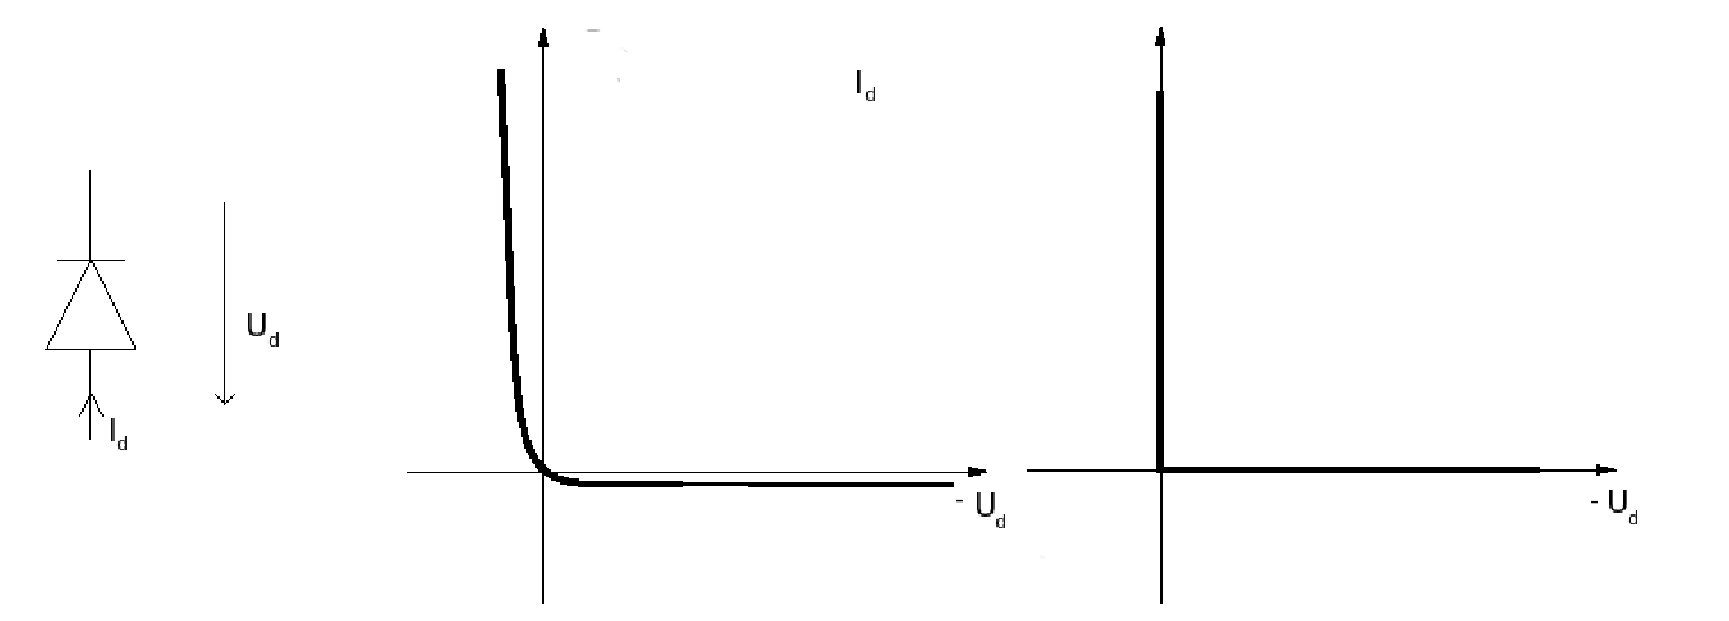
\includegraphics[width=100mm]{diode.eps}
  }
   \begin{block}{Branch Constitutive Equation of the diode:}
  \[ I_d =I_{s}(\exp{(-U_{D}/C)}-1)\]
  \end{block}
   \begin{block}{The complementary formulation:}
  \[0 \leq I_d \, \perp \, -U_{D} \geq 0\]
  \end{block}

}
\frame
{
  \frametitle{Ideal Transistor}
   \centerline{
  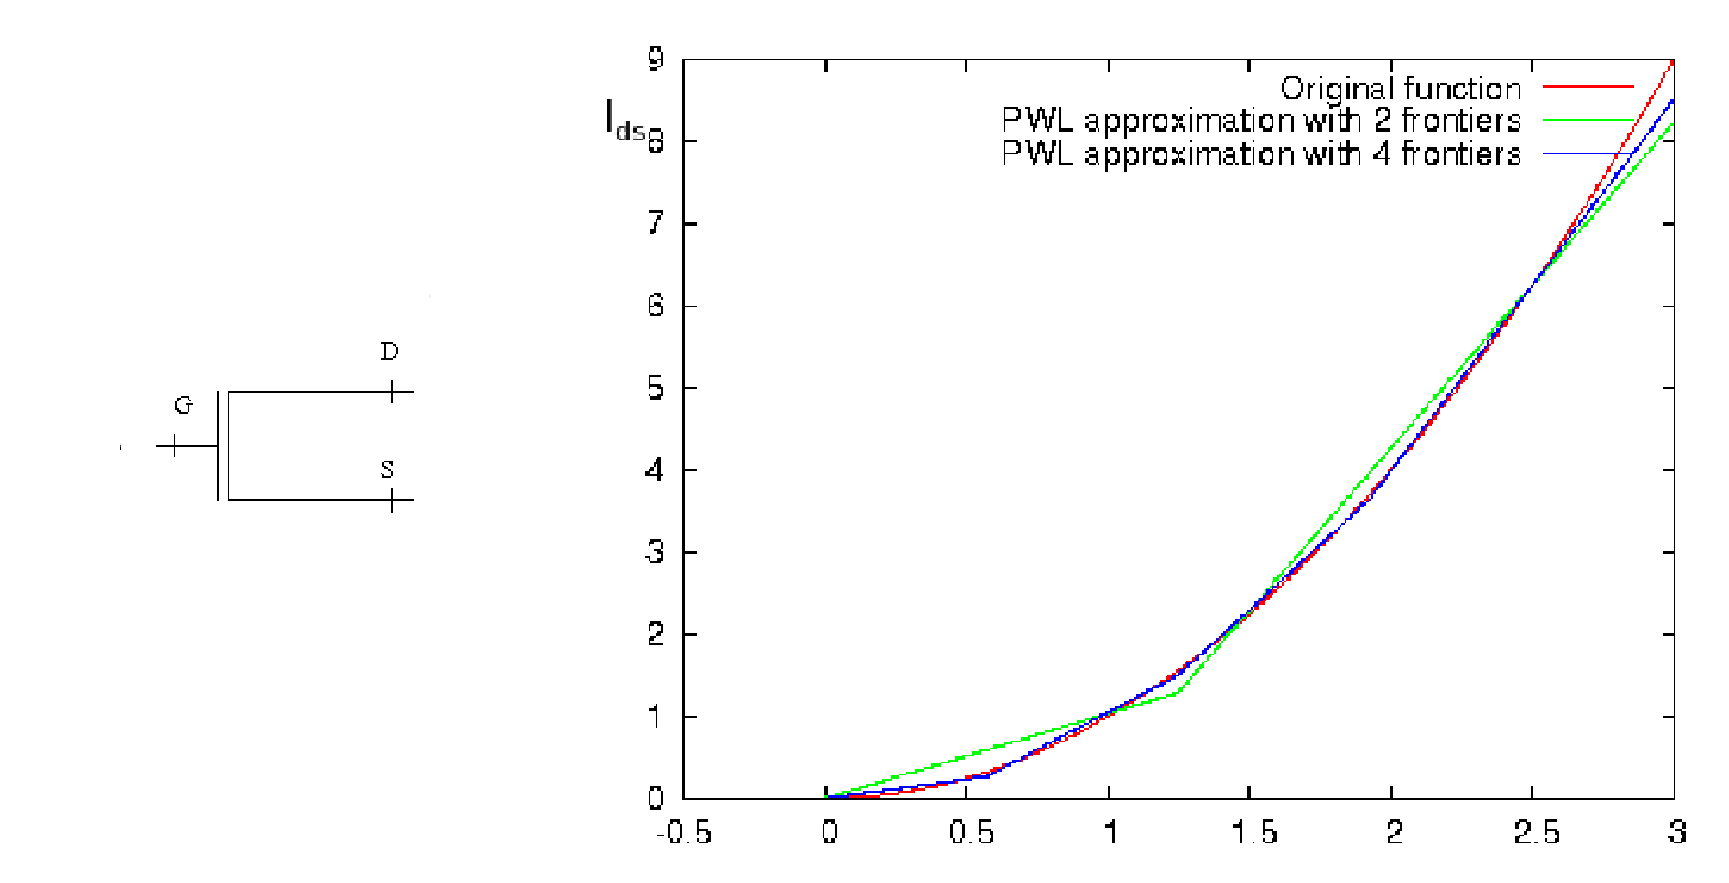
\includegraphics[width=100mm]{def2.eps}
  }
   \begin{block}{The complementary formulation:}
  \[ I_{d} = \left(\begin{array}{ccc}
  c_{1}&...&c_{10}\end{array}\right)\lambda \qquad  I_{d} = -I_{s}\]
  \[Y=A\left(\begin{array}{c}
  V_{d}\\
  V_{g}\\
  V_{s}\\\end{array}\right)+I\lambda + C\]
  \[0 \leq Y \, \perp \, \lambda \geq 0\]
  \end{block}

}

\section{Extend MNA for non-smooth components}

\frame
{
\frametitle{Extend MNA}
 It consists in replacing the Constitutive Equation of the non-smooth branch with the complementary
 formulation.

 \begin{block}{Unknowns}
 Before go ahead, the unknowns vector X is decomposed in:
\begin{itemize}
\item x which contains only the dynamic unknowns(currents in inductor and tensions from capacitor branches)
\item $Z_{s}$ which contains only the non dynamic unknowns(Voltage nodes,... ).
\end{itemize}
  \end{block}
  
 \begin{block}{A good choice of unknowns yields the following system:}
 
 \begin{eqnarray}
x'=A_{2x}x +A_{2zs}Z_{s} +R \lambda +A_{2s}&\label{eq2}\\
0=B_{2x}x+B_{2zs}Z_{s} + B_{2\lambda}\lambda + B_{2s}&\label{eq3}\\
Y=D_{2x}x+D_{2zs}Z_{s}+D_{2\lambda}\lambda + D_{2s} &\label{eq4}\\
0 \leq Y \, \perp \, \lambda \geq 0&\label{eqperp}
\end{eqnarray}

  \end{block}


}

%%% Local Variables: 
%%% mode: latex
%%% TeX-master: "main"
%%% End: 

\section{MLCS and MLCP}

\frame
{
\begin{block}{Mixed Linear Complementary System}
  Given the matrices   ${A_{x}} \in \RR^{n \times n}$, ${A_{z}} \in \RR^{n \times
  p}$, ${A_{v}} \in \RR^{n \times m}$, ${B_{x}} \in \RR^{p \times n}$, ${B_{z}} \in \RR^{p \times
  p}$, ${B_{v}} \in \RR^{p \times m}$, ${C_{x}} \in \RR^{m \times n}$, ${C_{z}} \in \RR^{m \times p}$,${C_{v}} \in \RR^{m \times m}$, and
  the vectors  $ {a} \in \RR^n$,$ {b}  \in \RR^p$,$ {c}  \in \RR^m$, the explicit MLCS denoted by
  $\mathrm{EMLCS}(A_{x},A_{z},A_{v},B_{x},B_{z},B_{v},C_{x},C_{z},C_{v},a,b,c)$ consists in finding three vectors $ {x}
  \in \RR^n$, $ {z} \in \RR^p$ and  $ {v} \in \RR^m$ such that
\begin{equation}\label{eq:mlcs2} 
  \begin{cases}
   x' = A_{x} x +A_{z} z +A_{v} v + a  \\
   0 = B_{x} x +B_{z} z + B_{v} v +b \\ \\
   {0} \le {v} \perp     C_{x} x+ C_{z}z +C_{v} v +c   \ge {0}
  \end{cases}.
\end{equation}
\end{block}
The time discretization of a MLCS leads to :
\begin{block}{Mixed Linear Complementary Problem}
  Given the matrices  ${A} \in \RR^{n \times n}$, ${B} \in \RR^{m \times m}$, ${C} \in \RR^{n \times m}$, ${D} \in \RR^{m \times n}$, and the vectors  $ {a} \in \RR^n, {b} \in \RR^m$, the MLCP denoted by $\mathrm{MLCP}(A,B,C,D,a,b)$ consists in finding two vectors $ {u} \in \RR^n$ and  $ {v} \in \RR^m$ such that
\begin{equation}\label{eq:mlcp1} 
  \begin{cases}
    A u + C v + a =0 \\  \\
    {0} \le {v} \perp     Du +B v +b   \ge {0}
  \end{cases}.
\end{equation}
\end{block}
At each step, SICONOS solves a MLCP.
}

\section{Solver MLCP}
\frame
{
  \frametitle{Mixed Linear Complementarity Problem solvers}

}

\frame
{
\frametitle{MLCP to linear system}
\begin{block}{ Given a MLCP}
 \begin{equation}\label{eq:mlcp1}
 \begin{cases}
M \left(\begin{array}{c}
   u\\
   \lambda
   \end{array}\right) + q = \left(\begin{array}{c}
   0\\
   y
   \end{array}\right) \\
      0 \le \lambda \perp     y   \ge 0

      \end{cases}
\end{equation}


\end{block}

\begin{block}{A linear system}

Let $I_\lambda$ and $I_y$, tow complementary subsets of $\{1,..,m\}$ and
looking for a solution such that : \\
\[
\begin{cases}
\lambda_i=0 \textrm{ for } i \in I_\lambda \\
 y_i=0 \textrm{ for } i \in I_y
\end{cases}
 \]




\[\textrm{Solve the linear system: }N \left(\begin{array}{c}
   u\\
   \lambda y
   \end{array}\right) = -q   \textrm{   With   }
   \begin{cases}
   N_{.i}=M_{.i} \textrm{ for } i \in \{1..n\}\\
   N_{.i}=M_{.i} \textrm{ for } i-n \in I_y\\
   N_{.i}=-e_{i} \textrm{ for } i-n \in I_\lambda
\end{cases}
\]
\[ \textrm { Solution if the complementarity hold: }
\begin{cases}
y_i \ge 0 \textrm{ for } i \in I_\lambda  \\
\lambda_i \ge 0 \textrm{ for } i \in I_y
\end{cases}
\]
An enumeratif algorithm consists in solving the $2^m$ cases.

\end{block}

}


\frame
{
\frametitle{A solver using the linear programming}
\begin{block}{ Given a MLCP}
 

\begin{equation}\label{eq:mlcp1}
 \begin{cases}
M \left(\begin{array}{c}
   U\\
   V
   \end{array}\right) + q = \left(\begin{array}{c}
   0\\
   W
   \end{array}\right) \\
      0 \le V \perp     W   \ge 0

      \end{cases}
\end{equation}


\end{block}

\begin{block}{An interesting linear programming problem}
Let I and J, tow subsets of \{1,..,m\} with  $I \cap J = \emptyset$

\begin{equation}\label{eq:mlcp1}
\begin{cases}
M \left(\begin{array}{c}
   U\\
   V
   \end{array}\right) + q = \left(\begin{array}{c}
   0\\
   W
   \end{array}\right)\\
V_i = 0 \textrm{ for } i \in I \qquad V_i \ge 0 \textrm{ for } i \notin I\\
W_j = 0 \textrm{ for } j \in J \qquad W_j \ge 0 \qquad j \notin J\\
\min{\sum_{i\notin I\cup J} V_i + \sum_{j\notin I\cup J} W_j}
\end{cases}
\end{equation}
Tow cases:\\
\begin{itemize}
 \item[--] The minimization doesn't success, it means the constraints are not compatible, $U_i =0 \textrm{ for } i \in I \qquad W_j=0 \textrm{ for } j\in J$ must be eliminated.\\
\item[--]Success, may the optimal point is a solution.
\end{itemize}

\end{block}

}

\frame
{
\frametitle{A branch and prune algorithm}
\[\left(\begin{array}{cccc}
4&0&0.2&0\\
0&2&0&0\\
1&0&0.2&0.5\\
0&0&0.5&0.2
 \end{array}\right) \left(\begin{array}{c}
 U_1\\
 U_2\\
 V_1\\
 V_2
 \end{array}\right) + \left(\begin{array}{c}
 -6\\
 -4\\
 -3\\
 2
 \end{array}\right) =  \left(\begin{array}{c}
 0\\
 0\\
 W_1\\
 W_2
 \end{array}\right) 
 \]
\begin{figure}[h]
\centerline{
 \scalebox{0.5}{
    \input{LP_step0.pstex_t}
 }
}
\end{figure}

}
\frame
{
\frametitle{A branch and prune algorithm}
\[\left(\begin{array}{cccc}
4&0&0.2&0\\
0&2&0&0\\
1&0&0.2&0.5\\
0&0&0.5&0.2
 \end{array}\right) \left(\begin{array}{c}
 U_1\\
 U_2\\
 V_1\\
 V_2
 \end{array}\right) + \left(\begin{array}{c}
 -6\\
 -4\\
 -3\\
 2
 \end{array}\right) =  \left(\begin{array}{c}
 0\\
 0\\
 W_1\\
 W_2
 \end{array}\right) 
 \]
\begin{figure}[h]
\centerline{
 \scalebox{0.5}{
    \input{LP_step1.pstex_t}
 }
}
\end{figure}

}
\frame
{
\frametitle{A branch and prune algorithm}
\[\left(\begin{array}{cccc}
4&0&0.2&0\\
0&2&0&0\\
1&0&0.2&0.5\\
0&0&0.5&0.2
 \end{array}\right) \left(\begin{array}{c}
 U_1\\
 U_2\\
 V_1\\
 V_2
 \end{array}\right) + \left(\begin{array}{c}
 -6\\
 -4\\
 -3\\
 2
 \end{array}\right) =  \left(\begin{array}{c}
 0\\
 0\\
 W_1\\
 W_2
 \end{array}\right) 
 \]
\begin{figure}[h]
\centerline{
 \scalebox{0.5}{
    \input{LP_step2.pstex_t}
 }
}
\end{figure}

}
\frame
{
\frametitle{A branch and prune algorithm}
\[\left(\begin{array}{cccc}
4&0&0.2&0\\
0&2&0&0\\
1&0&0.2&0.5\\
0&0&0.5&0.2
 \end{array}\right) \left(\begin{array}{c}
 U_1\\
 U_2\\
 V_1\\
 V_2
 \end{array}\right) + \left(\begin{array}{c}
 -6\\
 -4\\
 -3\\
 2
 \end{array}\right) =  \left(\begin{array}{c}
 0\\
 0\\
 W_1\\
 W_2
 \end{array}\right) 
 \]
\begin{figure}[h]
\centerline{
 \scalebox{0.5}{
    \input{LP_step3.pstex_t}
 }
}
\end{figure}

}
\section{Cost of the automatic equation formulation}

\frame
{
\frametitle{Cost evaluation}
Let
\begin{itemize}
\item $N_{b}$ the number of branches.
\item $N_{n}$ the number of nodes.
\item N = max\{$N_{b},N_{n}$\}
\end{itemize}

\begin{block}{The costs of the automatic circuit equation formulation:}

\begin{itemize}
\item To parse the Netlist : It consists in reading and storing the Netlist. O(N).
\item A topological analysis to build the unknowns vector:
The Minimum Spanning Tree algorithm complexity is O(Nlog(N))
\item Stamping method:
Each component writes its contribution in the table equation. O(N).
\item Matrix product:
Multiplied two dense matrices costs O($N^{3}$).
\end{itemize}
\end{block}


}

\section{Simulation}

\frame
{
\frametitle{Diodes Bridge}

\begin{figure}[h]
\centerline{
 \scalebox{0.3}{
    \input{Bridge.pstex_t}
 }
}\end{figure}
\begin {figure}[h]
 \scalebox{0.5}{
%GNUPLOT: LaTeX picture with Postscript
\begin{picture}(0,0)%
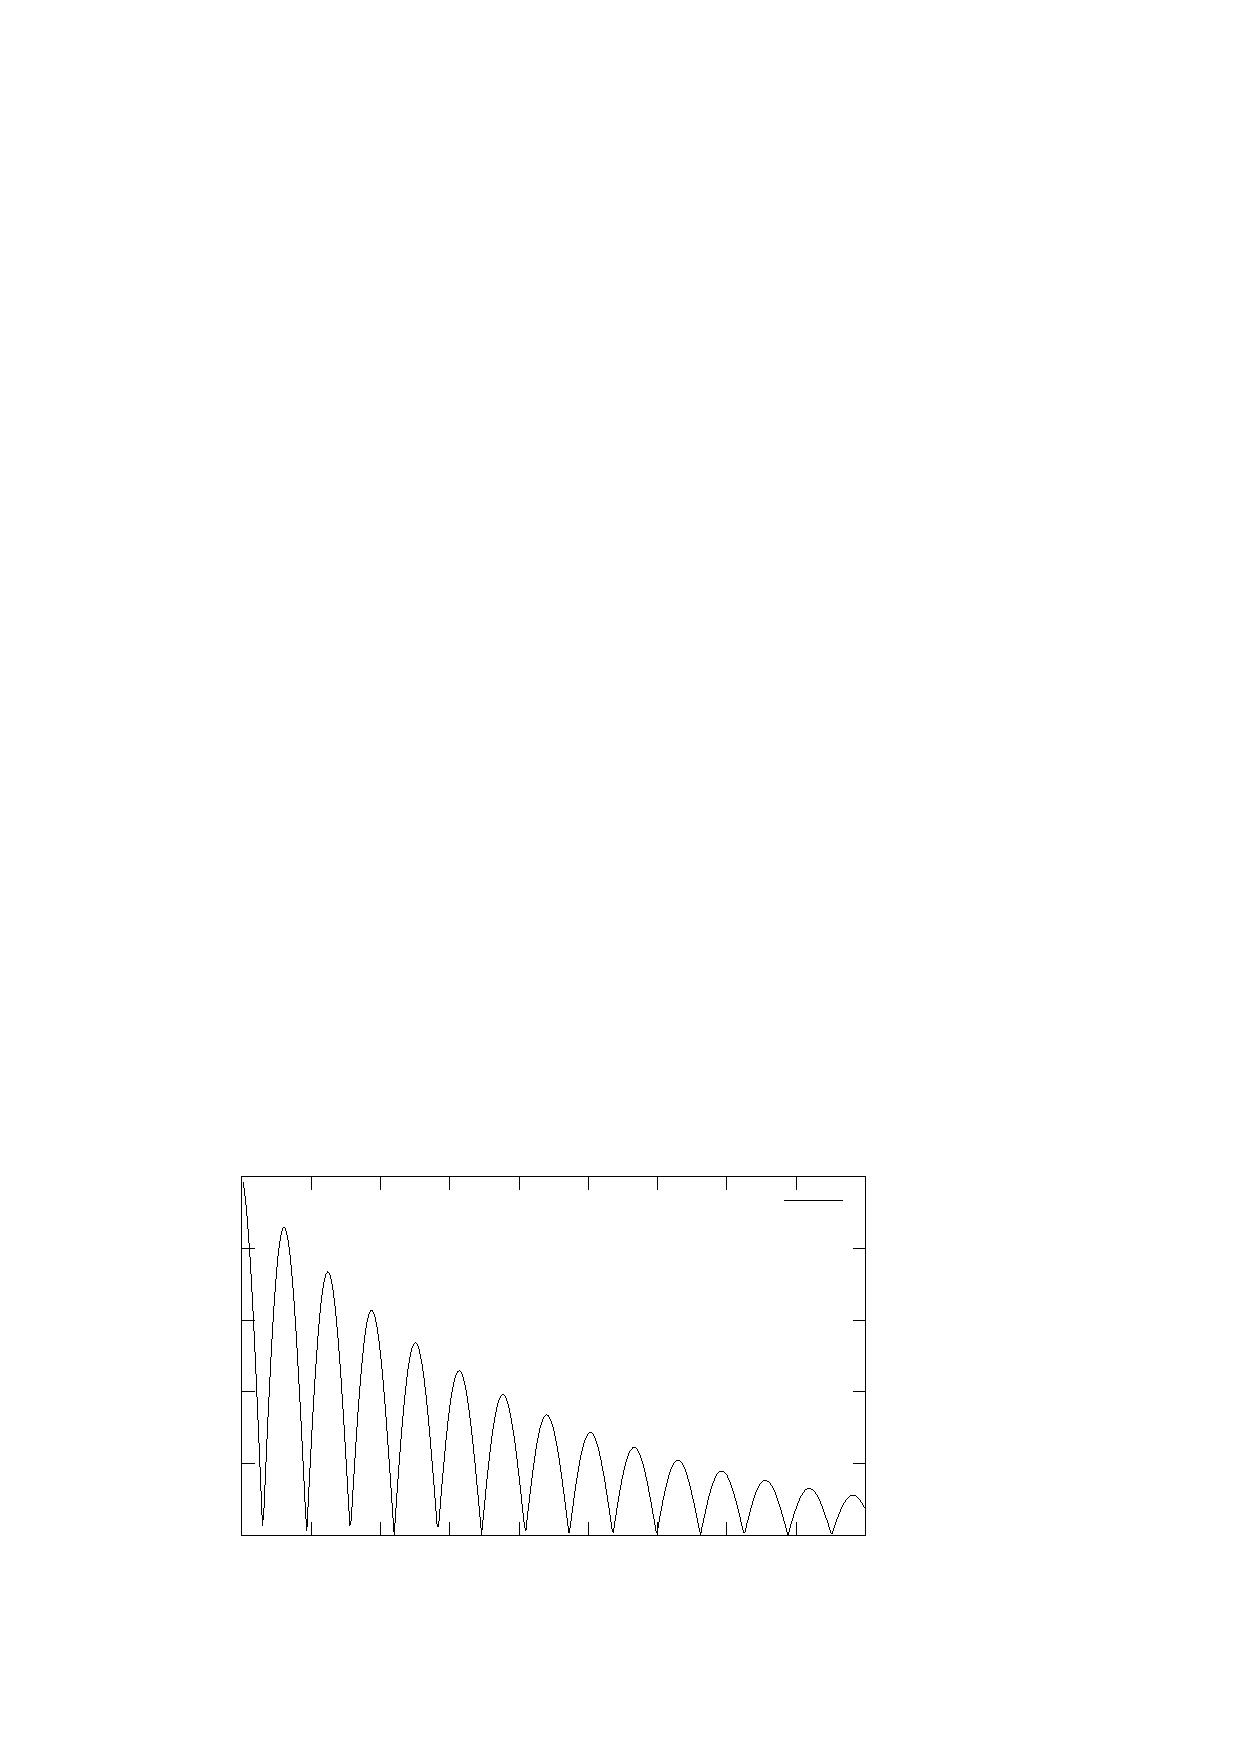
\includegraphics{diodes}%
\end{picture}%
\begingroup
\setlength{\unitlength}{0.0200bp}%
\begin{picture}(18000,10800)(0,0)%
\put(1925,1650){\makebox(0,0)[r]{\strut{} 0}}%
\put(1925,3370){\makebox(0,0)[r]{\strut{} 2}}%
\put(1925,5090){\makebox(0,0)[r]{\strut{} 4}}%
\put(1925,6810){\makebox(0,0)[r]{\strut{} 6}}%
\put(1925,8530){\makebox(0,0)[r]{\strut{} 8}}%
\put(1925,10250){\makebox(0,0)[r]{\strut{} 10}}%
\put(2200,1100){\makebox(0,0){\strut{} 0}}%
\put(3864,1100){\makebox(0,0){\strut{} 50}}%
\put(5528,1100){\makebox(0,0){\strut{} 100}}%
\put(7192,1100){\makebox(0,0){\strut{} 150}}%
\put(8856,1100){\makebox(0,0){\strut{} 200}}%
\put(10519,1100){\makebox(0,0){\strut{} 250}}%
\put(12183,1100){\makebox(0,0){\strut{} 300}}%
\put(13847,1100){\makebox(0,0){\strut{} 350}}%
\put(15511,1100){\makebox(0,0){\strut{} 400}}%
\put(17175,1100){\makebox(0,0){\strut{} 450}}%
\put(550,5950){\rotatebox{90}{\makebox(0,0){\strut{}U23}}}%
\put(9687,275){\makebox(0,0){\strut{}time e-5 s}}%
\put(14950,9675){\makebox(0,0)[r]{\strut{}'DiodeBridge.traj'}}%
\end{picture}%
\endgroup
\endinput

}
\end {figure} 

}
\frame
{
\frametitle{Buck converter}

\begin{figure}[h]
\centerline{
 \scalebox{0.5}{
    \input{buck.pstex_t}
 }
}\end{figure}
\begin {figure}[h]
 \scalebox{0.5}{
%GNUPLOT: LaTeX picture with Postscript
\begin{picture}(0,0)%
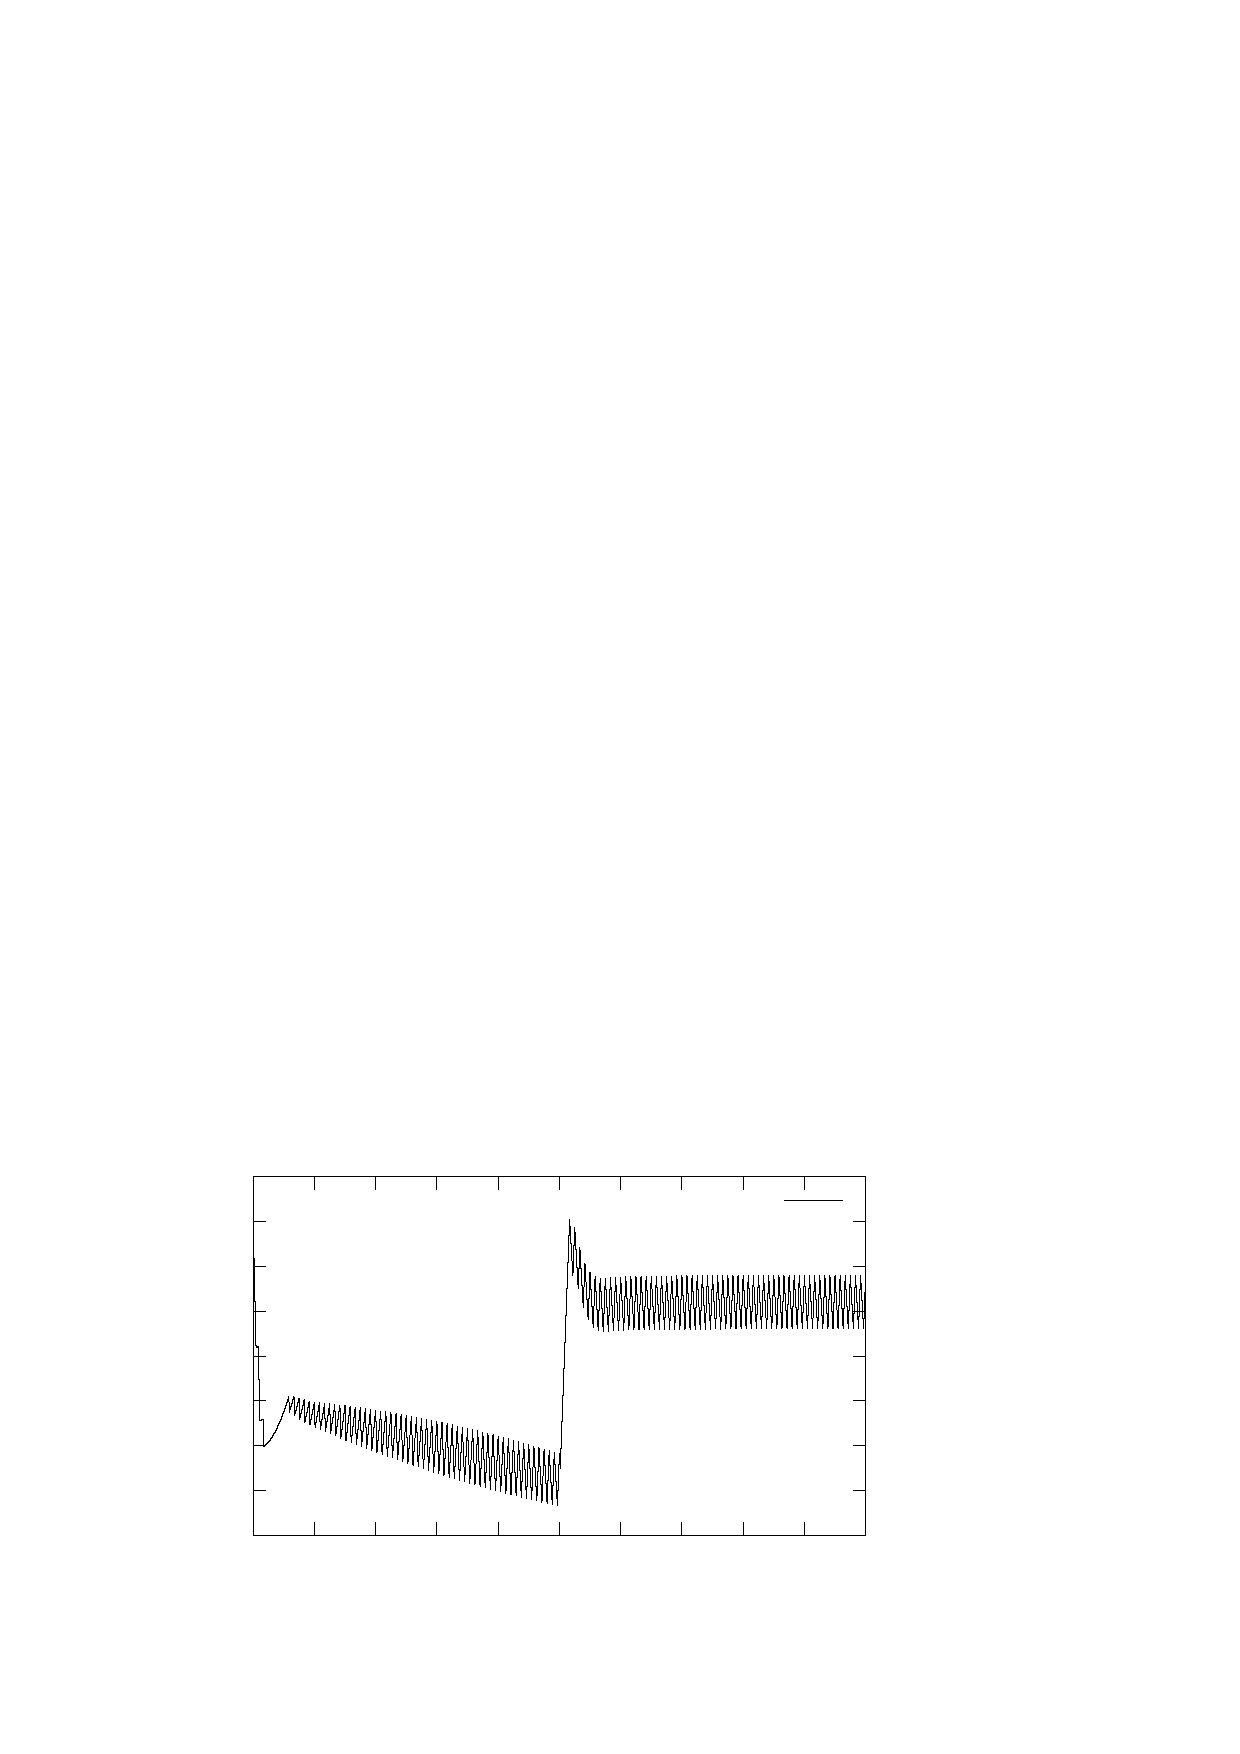
\includegraphics{Buck}%
\end{picture}%
\begingroup
\setlength{\unitlength}{0.0200bp}%
\begin{picture}(18000,10800)(0,0)%
\put(2200,1650){\makebox(0,0)[r]{\strut{}-0.7}}%
\put(2200,2725){\makebox(0,0)[r]{\strut{}-0.6}}%
\put(2200,3800){\makebox(0,0)[r]{\strut{}-0.5}}%
\put(2200,4875){\makebox(0,0)[r]{\strut{}-0.4}}%
\put(2200,5950){\makebox(0,0)[r]{\strut{}-0.3}}%
\put(2200,7025){\makebox(0,0)[r]{\strut{}-0.2}}%
\put(2200,8100){\makebox(0,0)[r]{\strut{}-0.1}}%
\put(2200,9175){\makebox(0,0)[r]{\strut{} 0}}%
\put(2200,10250){\makebox(0,0)[r]{\strut{} 0.1}}%
\put(2475,1100){\makebox(0,0){\strut{}   0}}%
\put(3945,1100){\makebox(0,0){\strut{}   2e-5}}%
\put(5415,1100){\makebox(0,0){\strut{}   4e-5}}%
\put(6885,1100){\makebox(0,0){\strut{}   6e-5}}%
\put(8355,1100){\makebox(0,0){\strut{}   8e-5}}%
\put(9825,1100){\makebox(0,0){\strut{}   1e-4}}%
\put(11295,1100){\makebox(0,0){\strut{}   1.2e-4}}%
\put(12765,1100){\makebox(0,0){\strut{}   1.4e-4}}%
\put(14235,1100){\makebox(0,0){\strut{}   1.6e-4}}%
\put(15705,1100){\makebox(0,0){\strut{}   1.8e-4}}%
\put(17175,1100){\makebox(0,0){\strut{}   2e-4}}%
\put(550,5950){\rotatebox{90}{\makebox(0,0){\strut{}Inductor current}}}%
\put(9825,275){\makebox(0,0){\strut{}time s}}%
\end{picture}%
\endgroup
\endinput

}
\caption{Buck converter simulation}
\end {figure} 

}
\section{Conclusion}

\frame
{
\begin{block}{The actual software version is able to parse and simulate a Netlist composed of:}
\begin{itemize}
\item Non constant sources.
\item Linear components : resistor, capacitor, inductance.
\item Non smooth components : Diode, Transistor, comparator.
\end{itemize}
\end{block}
\pause
\begin{block}{Perspectives}
\begin{itemize}
\item Topological analysis to index reduction of the DAE.
\item Multigrid algorithm: use a more simple picewise linear approximation.
\item Forecast active set: use a local piecewise linear approximation to solve a smaller MLCP.
\item Mixed Newton/MLCP simulator.
\item Specific electrical heuristics.
\item Improve the component model.
\end{itemize}
\end{block}

}



\def\newblock{}

\end{document}
%%% Local Variables: 
%%% mode: latex
%%% TeX-master: main
%%% End: 
